  \documentclass[twoside=false, %  doppelseitiger Druck
    DIV=15,% DIV Faktor für Satzspiegelberechnung, sie Doku zu KOMA Script
    BCOR=15mm, % Bindekorrektur
    chapterprefix=false,
    headinclude=true,
    footinclude=false,
    pagesize,%         write pagesize to DVI or PDF
    fontsize=11pt,%             use this font size
    paper=a4,%          use ISO A4
    bibliography=totoc,%         write bibliography-chapter to table of contents
    index=totoc,%         write index-chapter to table of contents
%    listof=totoc,
    cleardoublepage=plain,% \cleardoublepage generates pages with pagestyle empty
    headings=big,%       A4/B5
    listof=flat,%        improved list of tables
    numbers=noenddot
  ]{scrbook}


\usepackage{rotating} 
\usepackage{adjustbox}
\usepackage{afterpage} %landscape mode
\usepackage{pdflscape}
\usepackage{graphicx}
\usepackage[table,xcdraw]{xcolor}

\usepackage[utf8]{inputenc}
\usepackage{makeidx}
\usepackage{amsfonts}
\usepackage[slantedGreek,sc]{mathpazo}  % Schriftart Palatino
% \usepackage{lmodern}    % statt mathpazo, falls CM Fonts verwendet werden sollen
%\usepackage{mathptmx}    % statt mathpazo, falls Times  verwendet werden soll
\usepackage[scaled=.95]{helvet}
\usepackage{courier}
\usepackage[T1]{fontenc}
\usepackage{textcomp}
\usepackage{amsmath}            % standard math notation (vectors/sets/...)
\usepackage{bm}        % standard math notation (fonts)
\usepackage{fixmath}        % standard math notation (fonts)
\usepackage{graphicx}
\usepackage[facing=yes]{floatrow}       % mehrere Gleitobjekte nebeneinander/caption neben Bild/Tabelle
\usepackage[labelfont=bf,sf,font=small,labelsep=space,format=plain]{caption}
\usepackage{subcaption}
\usepackage{scrpage2}
% \usepackage{pstool}  % einbinden falls psfrag verwendet werden soll
\usepackage{epstopdf}
\usepackage[ngerman]{babel}
\usepackage{ellipsis}  % Korrigiert den Weißraum um Auslassungspunkte
\usepackage{microtype}  % optischer Randausgleich etc.
\usepackage
{acronym}  %Abkürzungsverzeichnis
\usepackage{xcolor}         % z.B. für schattierte Boxen
\usepackage{framed}			% shaded Umgebung
\definecolor{shadecolor}{gray}{.85}%

% Links im PDF
\usepackage[colorlinks=false,
            pdfborder={0 0 0},
            breaklinks=true]
            {hyperref}

\definecolor{bluekeywords}{rgb}{0,0,1}
\definecolor{greencomments}{rgb}{0,0.5,0}
\definecolor{redstrings}{rgb}{0.64,0.08,0.08}
\definecolor{xmlcomments}{rgb}{0.5,0.5,0.5}
\definecolor{types}{rgb}{0.17,0.57,0.68}

\usepackage{listings}
\usepackage{url}
\usepackage{footmisc}
\usepackage{chngcntr}





\counterwithout{footnote}{chapter}

\renewcommand{\lstlistingname}{Beispiel}% Listing -> Algorithm
\renewcommand{\lstlistlistingname}{\lstlistingname verzeichnis}%


\lstset{language=[Sharp]C,
	captionpos=b,
	%numbers=left, %Nummerierung
	%numberstyle=\tiny, % kleine Zeilennummern
	frame=lines, % Oberhalb und unterhalb des Listings ist eine Linie
	showspaces=false,
	showtabs=false,
	breaklines=true,
	showstringspaces=false,
	breakatwhitespace=true,
	escapeinside={(*@}{@*)},
	commentstyle=\color{greencomments},
	morekeywords={partial, var, value, get, set},
	keywordstyle=\color{bluekeywords},
	stringstyle=\color{redstrings},
	basicstyle=\ttfamily\small,
}


%\typearea[current]{calc}


% Einstellungen für Bild-/Tabellenbeschriftung neben dem Bild
\floatsetup[figure]{capbesideposition={inside,top}}
\floatsetup[table]{capbesideposition={inside,top},style=plaintop}
\renewfloatcommand{fcapside}{figure}[\capbeside][\FBwidth]
\newfloatcommand{tcapside}{table}[\capbeside][\FBwidth]

\lstdefinelanguage{Gherkin}{
	keywords={When, Then, Given, And},
	ndkeywords={Feature, Scenario},
	sensitive=false,
	comment=[l]{\#},
	morestring=[b]',
	morestring=[b]"
}

\newcommand*{\quelle}{% 
	\footnotesize Quelle: 
}
\selectlanguage{ngerman}


\deffootnote{1.5em}{1em}{%
 \makebox[1.5em][l]{\thefootnotemark}}

\makeindex

\newcommand{\real}{\mathord{\mathrm{I\!R}}}

\begin{document}
\selectlanguage{ngerman}
\def\figdir{figures}
\def\tabledir{tables}

\frontmatter

\pagestyle{scrplain}
\pagestyle{empty}

\begin{titlepage}

%\sf
\raggedleft

\vspace*{-2cm}


\includegraphics{\figdir/HS_Logo_aktuell_CMYK.eps}

\vfill

\centering
\LARGE
% \vspace*{\fill}
%-----------
Fakultät für Informatik  \vspace{0.5cm}\\
\Large
Studiengang Informatik

\vspace{2cm}

\LARGE

Containers with Machine Guns
\vspace{2cm}

\Large
Peter Kurfer, Marko Grgic, Sebastian Weißenbacher, Thomas Mildner\\
WS 2017/18

\vspace{1.5cm}

\vspace{1cm}

\flushleft
 \Large
\vspace*{\fill}

%-----------
\begin{tabbing}
Datum der Abgabe: \= tt.mm.jjjj \kill
Datum der Abgabe: \> 15. Januar 2018 \\
Prüfer: \> \ Hr.\ Frai\\
\end{tabbing}
%-----------

\end{titlepage}

\cleardoubleemptypage


%%% Local Variables: 
%%% mode: latex
%%% TeX-master: "d"
%%% End: 

\cleardoubleemptypage
%\chapter*{Kurzfassung}
\thispagestyle{empty}

\bigskip



\noindent

\vspace*{\fill}
Schlagworte: 
Container, Docker, Gatling,

\cleardoubleemptypage

\pagestyle{scrplain}
\pagenumbering{roman}
% ---------------------------------------------------
% D-TOC.TEX zur Verwendung mit TEXPART
% (an eigene Gegebenheiten anzupassen)
% ---------------------------------------------------
%
\tableofcontents
\cleardoublepage





\pagestyle{scrheadings}


\addtokomafont{caption}{\small}

\mainmatter

%\chapter{Wichtige Hinweise}
%\label{c:intro}
%
%Hier sind einige wichtige Hinweise zur Verwendung dieser Vorlage zusammengefasst, die erfahrungsgemäß oft falsch gemacht werden.
%Fehler bitte an jochen.schmidt@fh-rosenheim.de melden.
%
%
%%%%%%%%%%%%%%%%%%%%%%%%%%%%%%%%%%%%%%%%%%%%%%%%%%%%%%%%%%%
%\section{Abbildungen und Tabellen}
%\label{s:intro:abc}
%
%%Da dies leider immer wieder falsch gemacht wird (mit erheblichen Auswirkungen auf das Layout), hier einige Hinweise zur Positionierung von Bildern und Tabellen.
%%Im professionellen Textsatz werden diese als Gleitobjekte behandelt.
%%Wie der Name impliziert, bedeutet dies, dass Abbildungen (und Tabellen) relativ unabhängig vom Text platziert werden.
%%Insbesondere sollten Sie Latex \emph{niemals} dazu zwingen, Bilder genau an der von Ihnen vorgegebenen Stelle zu positionieren (z.\,B.\ mit Positionsangaben wie [h] oder schlimmer [h!]).
%%Es gibt dann für Latex keine Freiheit mehr, den Text richtig zu setzen, was unschöne Lücken zur Folgen hat.
%%Zudem wird durch ein Platzieren mitten im Text der Lesefluss unterbrochen.
%%
%%\begin{shaded*}
%%Gleitobjekte sollten daher immer mit [t] oder [tb] positioniert werden, oder bei großen Bildern auf Einzelseiten bzw.\ wenn mehrere Objekte auf einer textfreien Seite gesammelt werden sollen mit [p], alternativ mit [tbp].
%%\end{shaded*}
%%
%%Falls dadurch Bilder immer weiter vom eigentlichen Text wegrutschen, dann ist das ein Hinweise darauf, dass Sie im Verhältnis zu den Bildern zu wenig erläuternden Text geschrieben haben \dots
%%
%%Jede Abbildung erhält eine Abbildungsnummer und eine Bildunterschrift.
%%Diese sollte kurz beschreiben, was in der Abbildung zu sehen ist und zu verstehen sein, ohne dass man den gesamten Text gelesen hat.
%%Jede Abbildung wird im Text beschrieben und referenziert, und zwar über die Abbildungsnummer, also z.\,B.\  "`Wie in Abb.\ 3.1 zu sehen ist \dots"'.
%%Nicht zulässig ist z.\,B.\ "`Wie in der folgenden Abbildung zu sehen ist \dots"' -- es gibt keine "`folgende"' Abbildung!
%%Ferner sollte darauf geachtet werden, dass alle Abbildungen/Tabellen gut lesbar sind.
%%
%%
%%\begin{figure}[t]
%%\centering
%%
%%\begin{subfigure}{0.35\linewidth}
%%\centering
%%\includegraphics[width=\linewidth]{\figdir/handorig}
%%\caption{Originalbild}
%%\label{FIG:arexorig}
%%\end{subfigure}
%%\hspace{1cm}
%%\begin{subfigure}{0.35\linewidth}
%%\centering
%%\includegraphics[width=\linewidth]{\figdir/handaug}
%%\caption{erweitertes Bild}
%%\label{FIG:arexaugm}
%%\end{subfigure}
%%
%%\caption[AR Beispiel]
%%{Beispiel für Bilder, mit Beschreibung. Für nicht selbst erstellte Bilder, die nicht Public Domain sind, ist eine Quellenangabe erforderlich. Bilder aus \cite{Schmidt01:PAO}}
%%\label{FIG:arex}
%%\end{figure}
%%
%%Ein Beispiel wird in Abb.\ \ref{FIG:arex} gezeigt, mit zwei Teilen  bestehend aus Abb.\ \ref{FIG:arexorig} und \ref{FIG:arexaugm}.
%%Und ein Beispiel für das Einbinden einer Tabelle, zu sehen in Tabelle \ref{t:CodebookOverview}.
%%
%%\begin{table}[t]
%%\centering\small
%% \caption[Testtabelle]{Datenselektion für verschiedene Testdatensätze}
%%  \label{t:CodebookOverview}
%%\input{\tabledir/CodebookOverview.tex}
%%\end{table}
%%
%%Bei Bildern verwendet man üblicherweise eine Bildunterschrift (also caption  unter dem Bild), bei Tabellen steht die Beschriftung üblicherweise über der Tabelle, da diese von oben nach unten gelesen werden.
%%
%%Sind die Bilder/Tabellen schmal, kann die Beschriftung stattdessen auch neben dem Bild stehen.
%%Dies ist in Abb.\ \ref{fig:beschreibung-neben-bild} zu sehen (für ein Bild), verwendet wurde der Befehl fcapside.
%%Entsprechend funktioniert dies für Tabellen mit tcapside.
%%Die Einstellungen wurden so gewählt, dass die Beschriftung immer an der Innenseite ist (für doppelseitigen Druck).
%%Für eine korrekte Darstellung sind evtl.\ mehrere Latex-Läufe nötig.
%%
%%\begin{figure}[t]
%%\fcapside
%%{\caption{Beschreibung neben dem Bild mit fcapside. Für Tabellen wird tcapside verwendet}
%%\label{fig:beschreibung-neben-bild}}
%%{\includegraphics[width=0.35\textwidth]{\figdir/handorig}}
%%\end{figure}
%%
%%\begin{figure}[t]
%%\fcapside
%%{\caption{Beschreibung neben dem Bild mit fcapside. Für Tabellen wird tcapside verwendet}
%%\label{fig:beschreibung-neben-bild-2}}
%%{\includegraphics[width=0.35\textwidth]{\figdir/handorig}}
%%\end{figure}
%%
%%
%%\section{Seitenumbrüche}
%%Überlassen Sie Seitenumbrüche Latex, verwenden Sie kein newpage oder pagebreak.
%%Diese Befehle sind nur in sehr wenigen Ausnahmefällen erforderlich.
%%Wenn Sie diese verwenden müssen ist dies eher ein Hinweis darauf, dass etwas anderes mit Ihrem Layout nicht stimmt.
%%
%%\section{Schriftart}
%%Als Schriftart für den Haupttext ist Palatino voreingestellt.
%%Dies hat in erster Linie zwei Gründe:
%%\begin{enumerate}
%%\item
%%Die Schrift ist etwas breiter als z.\,B.\ Times und daher gerade für den A4-Druck (zur besseren Lesbarkeit) noch am besten geeignet.
%%\item
%%Es gibt einen passenden Mathematikzeichensatz dazu, d.\,h.\ Ziffern und Buchstaben (wenn beide gerade bzw.\ kursiv gedruckt werden) sehen im Text und im Mathemodus gleich aus -- alles andere wäre unschön.
%%\end{enumerate}
%%Passende Mathematikzeichensätze gibt es auch für Times und Computer/Latin Modern, die stattdessen verwendet werden können.
%%Kommentieren Sie in diesem Fall das Paket mathpazo (durch ein \%) aus, und dafür lmodern (für Latin Modern) oder mathptmx (für Times) ein.
%%
%%Weitere Hinweise zu den Themen Seitenlayout/Einfluss der Schriftart findet man z.\,B.\ in der Dokumentation zu KomaScript\footnote{\url{http://www.komascript.de}}.
%%
%
%\section{Druck}
%Die Vorlage ist für doppelseitigen Druck eingerichtet, den Sie auch verwenden sollten.
%Wenn (aus welchem Grund auch immer) ein einseitiger Druck erwünscht ist, schalten Sie die Vorlage bitte um: Ganz oben in thesis.tex muss dann aus twoside=true ein twoside=false werden.
%Wird dies  nicht beachtet erscheinen die Seitenzahlen einmal innen und einmal außen, zudem entstehen komplett leere Seiten (die beim doppelseitigen Druck Rückseiten wären, die dazu dienen, dass ein neues Kapitel auf einer rechten Seite anfängt).
%Wenn Sie die Arbeit nicht selbst drucken, denken Sie daran, den Dienstleister auf den doppelseitigen Druck hinzuweisen.
%
%
%
%\section{Dokument Richtlinien}
%Beachten Sie bitte auch die Hinweise im separaten Dokument "`Hinweise zur Erstellung von Abschlussarbeiten"'.
%
%\section{Diverse Beispiele}
%
%Verwenden Sie für Querverweise den Befehl label und  ref (Bilder und Tabellen), eqref (Formeln), pageref (Seitenzahlen) damit diese automatisch erzeugt werden.
%Beachten Sie vor der Abgabe der Arbeit, dass evtl.\ mehrere Latexläufe erforderlich sind, bis alle Querverweise korrekt sind, da Latex diese während eines Laufs erzeugt und beim nächsten wieder einliest.
%Durch Verschiebungen können je nach verwendeten Paketen auch drei oder vier Läufe erforderlich sein, bis alles passt.
%
%
%
%Beispiel für eine Formel
%\begin{equation}
%\label{eq:cvp:test}
%f(x) = \frac{1}{3} x + 5, \quad x \in \real.
%\end{equation}
%
%Und noch eine:
%\begin{equation}
%\label{eq:cvp:matvec}
%\bm{M}  = \bm{Ax} \pi, \quad \bm{A} \in \real^{2 \times 2}, \bm{x} \in \real^2.
%\end{equation}

%Eine Referenz auf eine Formel: \eqref{eq:cvp:test}.

%Und eine Literaturreferenz: \cite{Auer00:HTF}.
%Verwenden Sie auf jeden Fall Bibtex (oder etwas äquivalentes), Referenzen sollten auf keinen Fall manuell eingefügt werden.
%
%Gedankenstriche entstehen durch zwei Minuszeichen -- und sind länger als ein Bindestrich -.
%
%Und wenn es ganz besonders schön aussehen, dann beachten Sie zusätzlich
%\begin{itemize}
%\item Der Leerraum nach eine Punkt am Satzende ist größer als der nach einer Abkürzung (wie evtl.). 
%Um Latex zu sagen, dass der Punkt kein Satzende ist, wird dieser bei Abkürzungen durch einen Backslash markiert, also so: evtl.\textbackslash, ohne Leerzeichen zwischen Punkt und Backslash.
%
%\item
%Leerräume zwischen zwei Teilen einer Abkürzung (wie z.\,B.) sind kleiner als zwischen einzelnen Wörtern, außerdem sollten diese beiden Buchstaben nicht getrennt werden. Dies erreicht man durch: z.\textbackslash,B.\textbackslash, wieder ohne Leerzeichen.
%\end{itemize}
%Noch ein Hinweis zur Silbentrennung von Wörtern mit Bindestrichen: Diese werden nur direkt am Bindestrich getrennt (so soll es eigentlich sein), was insbesondere im Deutschen oft dazu führt, dass Wörter in den Rand hineinragen (man bekommt auch eine Overfull Box Warnung).
%Möchte man, dass die Wörter selbst auch getrennt werden dürfen, so kann man
%\begin{itemize}
%\item
%entweder bei Problemfällen manuelle Trennpunkte durch \textbackslash - in das Wort einfügen,
%\item oder statt des Bindestrichs - die Zeichenfolge "'= verwenden, also wort"'=wort statt wort-wort.
%\end{itemize}
%In vielen Fällen sollte man sich zudem fragen, ob das Wort nicht eher zusammen geschrieben werden sollte (statt des Bindestrichs).
%
%
% Local Variables: 
% mode: latex
% TeX-master: "thesis.tex"
% End: 

\chapter*{Kurzfassung}
\thispagestyle{empty}

\bigskip



\noindent

\vspace*{\fill}
Schlagworte: 
Container, Docker, Gatling,

\chapter{Einleitung}

Dies ist eine \ac{Demo}.

Hier ist es nur noch \ac{Demo}

\chapter{Docker}
\label{c:docker}

Zu Beginn ist es notwendig, die Grundlagen von Docker zu verstehen.
Hierfür bietet dieses Kapitel einen Einblick in die wichtigsten Begrifflichkeiten, die Architektur und die für diese Arbeit notwendigen Funktionalitäten.
Falls nicht anders gekennzeichnet basiert dieses Kapitel auf der offiziellen Dokumentation von Docker \cite{Docker:online1}.

\section{Einführung in Docker}
\label{c:einführung}

\begin{figure}
	\centering
	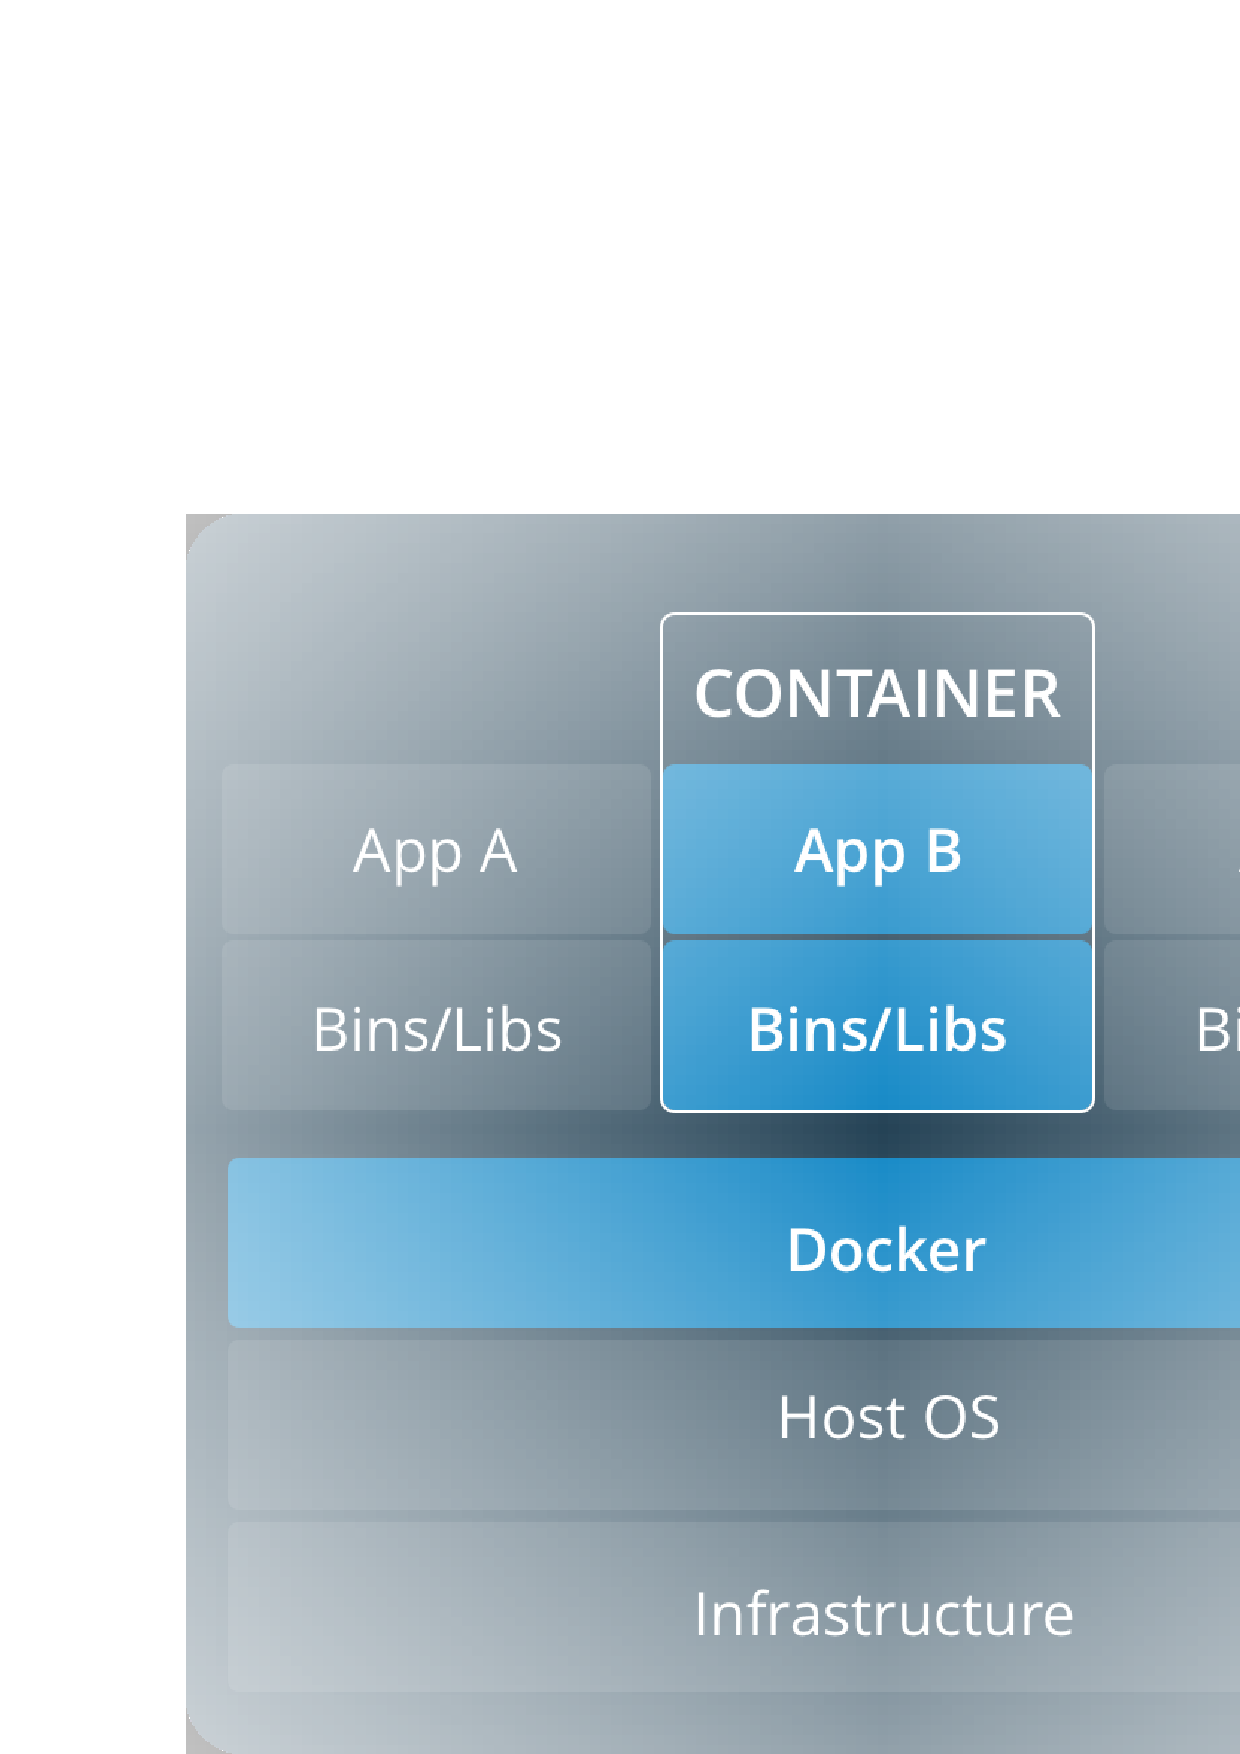
\includegraphics[width=0.7\linewidth]{figures/Docker}
	\caption[Betriebssystem basierte Virtualisierung mit Docker-Containern]{Umsetzung einer Betriebssystem basierten Virtualisierung mit Docker-Containern}
	\label{fig:docker}
	\tiny{\quelle\url{https://www.docker.com/what-container}}
\end{figure}

\begin{figure}
	\centering
	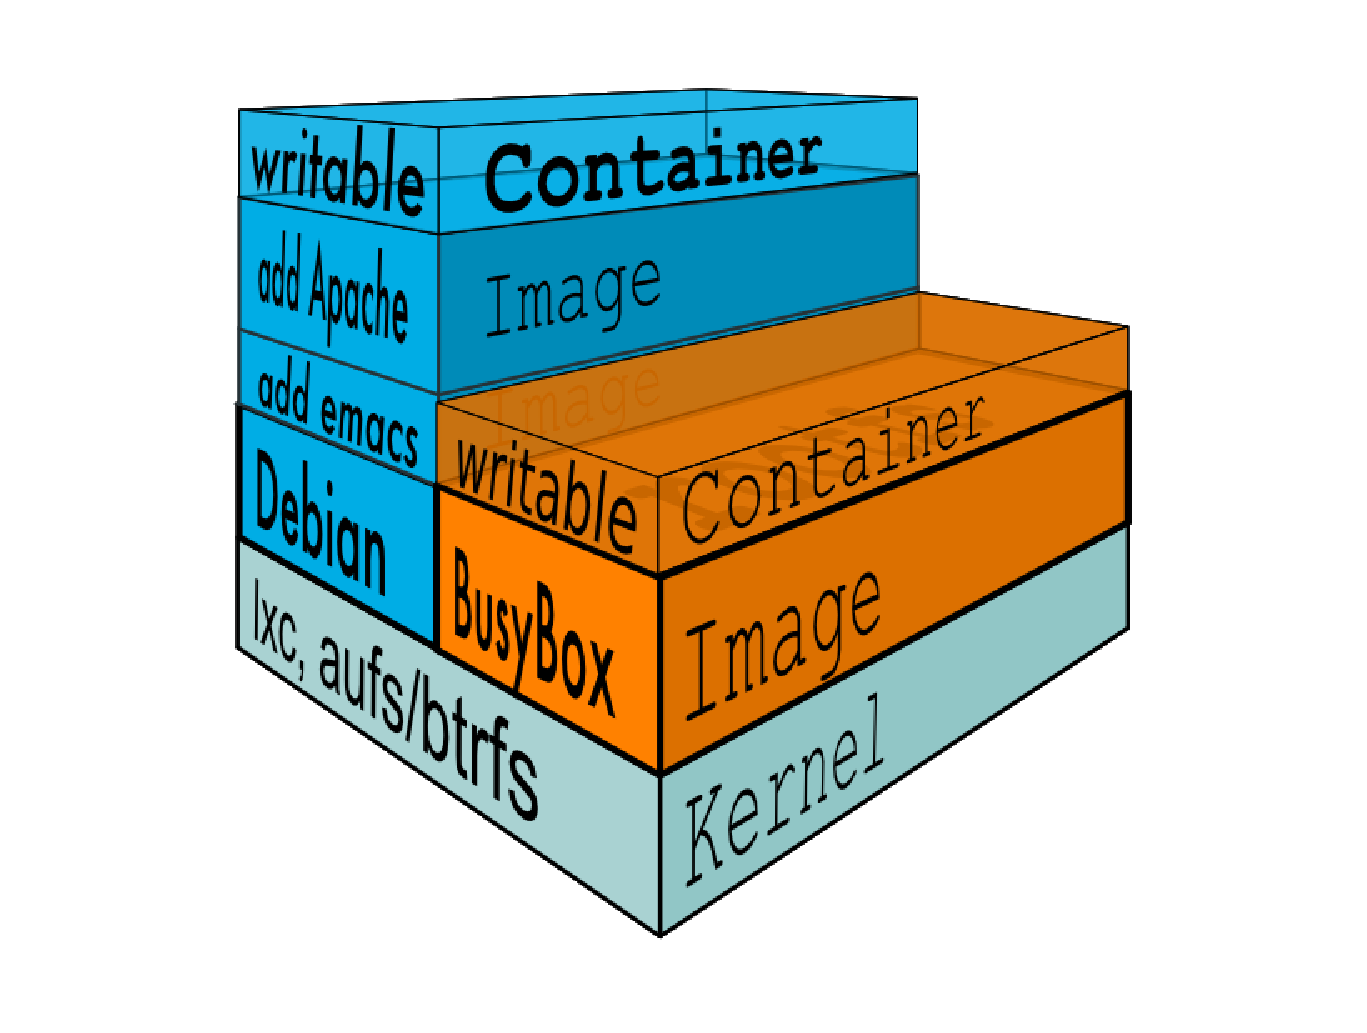
\includegraphics[width=0.7\linewidth]{figures/DockerLayer}
	\caption[Aufbau von Docker mittels Schichten]{Aufbau von Docker mittels Schichten}
	\label{fig:dockerlayer}
	\tiny{\quelle\url{https://blog.docker.com/2015/10/docker-basics-webinar-qa/}}
\end{figure}

Bei Docker handelt es sich um eine containerbasierte Virtualisierung.
Es ist möglich, die Docker-Container sowohl auf einem Windows-System, Unix-System, in der Cloud oder sogar in einer virtuellen Maschine auszuführen.
Hierfür wird, wie in Abbildung \ref{fig:docker} gezeigt, in einem Host Betriebssystem die Docker Runtime zur Verfügung gestellt sowie mehrere Docker-Container ausgeführt.
Die Docker Runtime übernimmt die Verwaltung der einzelnen Docker-Container, die die benötigten Binaries, Bibliotheken und Anwendungen enthalten.

Im Vergleich zur Virtualisierung mittels einer \ac{VM} bieten Docker-Container einige Vorteile.
Hierzu zählen einerseits der geringere Bedarf an CPU und RAM sowie andererseits die schnelle Startgeschwindigkeit eines Docker-Containers im Vergleich zu einer herkömmlichen \ac{VM}.

Trotz dessen, dass sich die Docker-Container, wie in Abbildung \ref{fig:docker} abgebildet, einen Betriebssystemkernel teilen, sind diese vollständig voneinander isoliert, was dazu führt, dass sich Docker-Container besonders für Continuous Integration und Development eignen.
Dies ist möglich, da die Workspaces, in Docker \glqq{}Container\grqq{} genannt, auf Linux Containern basieren und somit zur Isolierung die folgenden Namespaces genutzt werden:

\begin{itemize}
	\item \textit{ipc}-Namespace zur Verwaltung der Interprozess Kommunikationsressourcen (Shared Memory)
	\item \textit{mnt}-Namespace zur Verwaltung des Dateisystems
	\item \textit{net}-Namespace zur Verwaltung des Netzwerk Interfaces
	\item \textit{pid}-Namespace zur Isolation von Prozessen
	\item \textit{uts}-Namespace zur Isolation des Kernels und der Versions Identifier
\end{itemize}

Zur Kontrolle der Hardware Ressourcen verwendet Docker die von Linux stammenden \ac{cgroups}.
Mittels dieser ist es möglich, den Containern Hardware Ressourcen zuzuweisen und diese nötigenfalls, wie z. B. den RAM, zu beschränken.

Neben den oben genannten Funktionen nutzt Docker mit dem \ac{UnionFS} eine weitere Linux Funktion.
Hierbei wird, wie in Abbildung \ref{fig:dockerlayer} zu sehen, auf dem Boot Dateisystem (Kernel) ein Dateisystem Stack erzeugt, der aus mehreren read-only Layern, die Images genannt werden, besteht.
Jedes Image referenziert und beinhaltet lediglich Ergänzungen zum vorherigen Image.
Dies macht Docker leichtgewichtig und schnell und ermöglicht einen im Vergleich zu traditionellen \acp{VM} höheren operativen Workload auf der gleichen Hardware.

Beim Start von Docker wird, wie in Abbildung \ref{fig:dockerlayer} dargestellt, ein read-write Layer auf dem Stack erzeugt.
In diesen werden die notwendigen Dateien der darunterliegenden Images kopiert (\textit{copy-on-write}), dort nötigenfalls umgeschrieben und abgelegt.
Wird Docker gestoppt, so wird der writable Layer und damit auch sämtliche Änderungen an den Dateien gelöscht, falls nicht ein Speichervolumen außerhalb des \ac{UnionFS} angebunden wurde.
Somit ist es möglich, die Docker-Container immer zu den gleichen Bedingungen zu starten.

\section{Architektur}
\label{c:architektur}

Wird die Docker Architektur betrachtet, so zeigt die Abbildung \ref{fig:dockerengine}, dass es sich bei der Docker Runtime oder auch Docker-Engine lediglich um eine Client-Server-Architektur mit mehreren Hauptkomponenten handelt.

Im Kern der Docker-Engine befindet sich, wie in Abbildung \ref{fig:dockerengine} gezeigt, der Server oder auch Docker Daemon.
Dieser erstellt und verwaltet einerseits die Docker-Container, Images, Netzwerke und Dateisysteme und er ist andererseits in der Lage, mit anderen Docker Daemons zu kommunizieren.
Mittels einer REST-API und dem \ac{CLI} ist der Client im Stande, mit einem oder mehreren Docker Daemons zu interagieren und diesen, per \ac{CLI} Kommandos oder mit Hilfe von Skripten, Aufträge zu erteilen.

Ein weiterer wichtiger Bestandteil der Docker Architektur sind, wie in Abbildung \ref{fig:dockerarchitecture} zu sehen, die Docker Registries.
Hierbei wird zwischen privaten und öffentlichen Registries unterschieden.
Die wichtigsten öffentlichen Registries sind der Docker Hub und die Docker Cloud.
So wird z. B. mittels der Befehle \textit{docker run} oder \textit{docker pull} per default das Standard Image vom Docker Hub genutzt, um den Container über dem Dateisystem Stack automatisch zu bauen.

Jedes Image in einer Docker Registry verfügt über einen sogenannten \textit{Tag}.
Das Standard Image wird markiert durch den Tag \textit{latest}.
Durch Tags ist es möglich unterschiedliche Versionen eines Containers unter dem selben Namen zu gruppieren.
Beispielsweise gibt es den offiziellen Java-Container sowohl mit JDK 7, 8 oder 9 und mit JRE 7, 8 oder 9.

Des Weiteren besteht die Möglichkeit, mit Hilfe des \ac{DDC} eigene (private) Registries anzulegen und z. B. mittels des \textit{docker push} Kommandos eigene Images in den neu angelegten Registries abzulegen und später für den Buildprozess zu nutzen.

\begin{figure}
	\centering
	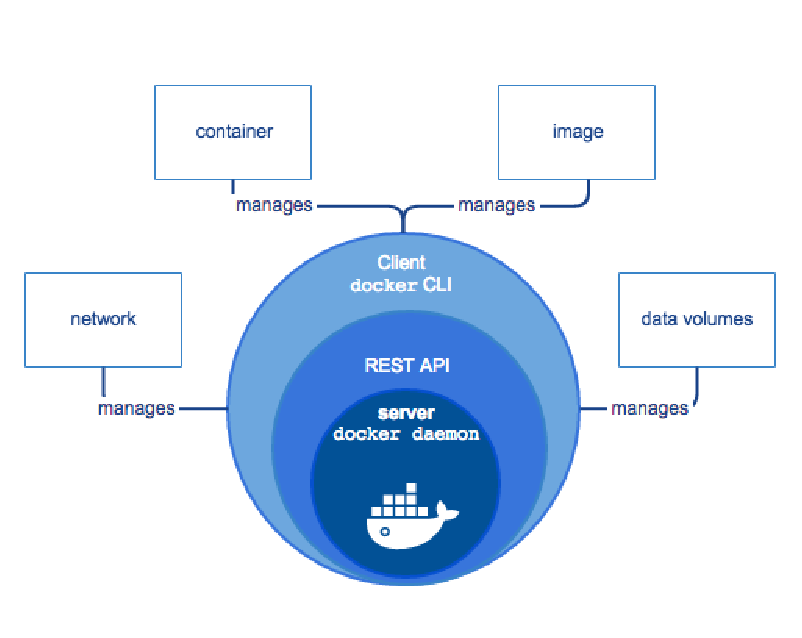
\includegraphics[width=0.7\linewidth]{figures/DockerEngine}
	\caption[Aufbau Docker-Engine]{Schematische Darstellung des Aufbaus der Docker-Engine}
	\label{fig:dockerengine}
	\tiny{\quelle\url{https://docs.docker.com/engine/docker-overview/}}
\end{figure}

\begin{figure}
	\centering
	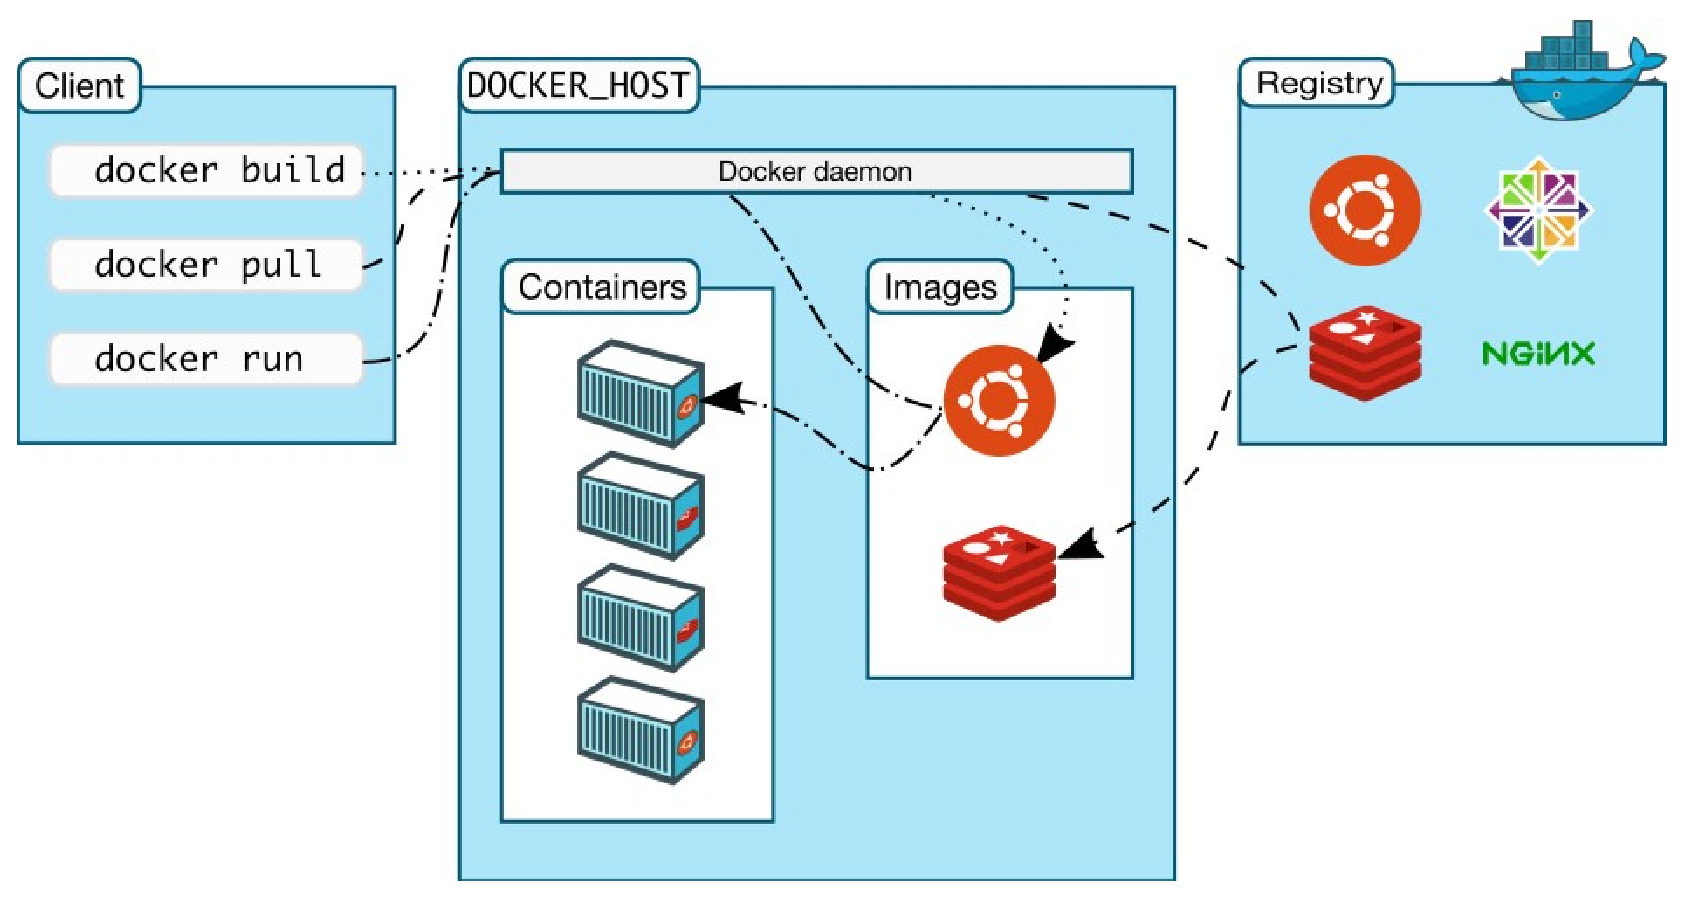
\includegraphics[width=0.7\linewidth]{figures/DockerArchitecture}
	\caption[Detailansicht der Docker-Architektur]{Detailansicht der Docker-Architektur}
	\label{fig:dockerarchitecture}
	\tiny{\quelle\url{https://docs.docker.com/engine/docker-overview/}}
\end{figure}

\section{Docker Funktionalitäten}
\label{c:funktionalität}

Im folgenden Unterkapitel werden die für diese Arbeit wichtigsten Docker Funktionalitäten erläutert.
Hierbei wird, falls notwendig anhand einer Begründung erklärt, weshalb eine bestimmte Ausprägung einer Funktionalität gewählt wurde.

\subsection{Docker-Compose}
\label{ss:dockerCompose}

Standardmäßig wird jeder Docker-Container einzeln mit dem Kommando \textit{docker run} erstellt und ausgeführt.
Betrachtet man den Titel dieser Arbeit, "Containers with Machine Guns", so geht daraus hervor, dass es sich nicht zwingend um einen einzelnen Container handelt, sondern möglicherweise um eine Vielzahl von Containern.
Diese sollen nach Möglichkeit alle gleichzeitig gestartet und ausgeführt werden.

Um dies zu erreichen, bietet Docker Docker-Compose an.
Hierbei handelt es sich um ein Tool von Docker, mit dem es möglich ist, einen Service für eine Anwendung zu konfigurieren und diese sowie die dazugehörigen Container anschließend mit einem einzigen Befehl zu starten.

Hierfür wird zu Beginn ein Dockerfile erstellt, mit dem es möglich ist, die Images und Container einfach zu vervielfältigen.
Im Anschluss daran wird die YAML-Datei docker-compose.yml genutzt, um den Service zu definieren.
Code-Beispiel \ref{dockerComposeFile} zeigt, wie in dieser Datei z. B. die zwei Services \textit{web} und \textit{redis} definiert werden.
Des Weiteren wird dargestellt, wie der Service \textit{web} im Punkt \textit{build} das Dockerfile aus dem aktuellen Verzeichnis und der Service \textit{redis} das öffentliche Redis Image \glqq{}redis:alpine\grqq{} des Docker Hub verwendet.
Zusätzlich ist ersichtlich, dass der Service \textit{web} über den Default-Port 5000 des Flask Web-Servers erreichbar ist.
Mittels des Kommandos \textit{docker-compose up} wird anschließend die gesamte Anwendung anhand der Docker-Compose-Datei gestartet.

\begin{minipage}{\linewidth}
	\begin{lstlisting}[frame=single,caption=Beispiel Docker Compose Datei \cite{Docker:online2}, label=dockerComposeFile, language=Scala]
	version: '3'
	services:
	  web:
	    build: .
	    ports:
	     - "5000:5000"
	  redis:
	    image: "redis:alpine"
	\end{lstlisting}
\end{minipage}

Mit Hilfe von Docker-Compose ist es neben dem Starten des Service möglich, diesen zu stoppen, erneut zu bauen und Befehle an einzelne Container des Service zu senden.
Des Weiteren ermöglicht Docker-Compose die Statusabfrage sowie das Auslesen von Logs eines laufenden Service.

\subsection{Netzwerke}

Dieser Abschnitt des Kapitels zeigt die default Netzwerke und die Möglichkeiten zum Definieren eines eigenen Netzwerkes in Docker auf.
Hiermit soll erläutert werden, wie der angelegte Service außerhalb des Host-Systems verfügbar gemacht wird.

\subsubsection{Default Netzwerke}

Mit der Installation von Docker werden standardmäßig die folgenden drei Netzwerke erzeugt:

\begin{itemize}
	\item None-Netzwerk
	\item Host-Netzwerk
	\item Bridge-Netzwerk
\end{itemize}

Das None-Netzwerk ermöglicht es, einen Container zu einem spezifischen Netzwerk Stack hinzuzufügen, allerdings besitzt dieser Container kein eigenes Netzwerk-Interface. 
Mit Hilfe des Host-Netzwerkes wird der Container zum Netzwerk Stack des Host Systems hinzugefügt.
Dies hat zur Folge, dass keine Isolation zwischen dem Host System und den Containern mehr gegeben ist.
Des Weiteren sind sowohl das None als auch das Host-Netzwerk nicht direkt mit Docker konfigurierbar.

Das dritte default Netzwerk, das Bridge-Netzwerk, ist auf allen Host Systemen von Docker vorhanden.
Wird kein alternatives Netzwerk definiert, so wird jeder neu erstellte Container automatisch an dieses gekoppelt.
Die angebundenen Container wären zwar durch \textit{Port Mapping} und mit Hilfe von IP-Adressen, aber nicht mit den Container-Namen per DNS-Auflösung, in der Lage, miteinander zu kommunizieren, aber dieses Vorgehen wird für das default Bridge-Netzwerk von Docker nicht empfohlen.
Stattdessen sollte für derartige Anwendungsfälle das, im Abschnitt User definierte Netzwerke, beschriebene Bridge-Netzwerk verwendet werden.

\subsubsection{User definierte Netzwerke}

Zur Erstellung eines User definierten Netzwerks bietet Docker entsprechende Treiber an.
Mit diesen ist es möglich, die folgenden Netzwerke anzulegen:

\begin{itemize}
	\item User definierte Bridge-Netzwerke
	\item Overlay-Netzwerke
	\item MACVLAN-Netzwerke
\end{itemize}

Wenn keines der gelisteten Netzwerke dem Anwendungsfall entspricht, so besteht die Möglichkeit, ein eigenes Plugin für einen Netzwerk-Treiber zu erstellen.
Eine genaue Beschreibung hierfür sowie für das oben gelistete MACVLAN-Netzwerk würde für diese Arbeit zu weit gehen, weshalb diese an dieser Stelle nur zum Zweck der Vollständigkeit erwähnt werden.

Das User definierte Bridge-Netzwerk bietet mit Hilfe des eingebetteten DNS-Server des Docker Daemon eine DNS-Auflösung.
Des Weiteren besteht optional die Möglichkeit zur Steuerung der Kommunikation der sich auf einem Host-System und in einem Netzwerk befindlichen Container.
Diese können an kein oder jederzeit, auch während der Ausführung eines Containers, an ein oder mehrere Netzwerke angeschlossen oder von diesen getrennt werden.
Ist dies nicht erforderlich, so sind alle Container ohne weitere Konfiguration in der Lage, mit jedem beliebigen Container des Netzwerkes zu kommunizieren.
Hieraus geht hervor, dass das Netzwerk die darin befindlichen Container vollständig, wie in Abbildung \ref{fig:dockerportpuex} zu sehen, isoliert.

\begin{figure}[H]
	\centering
	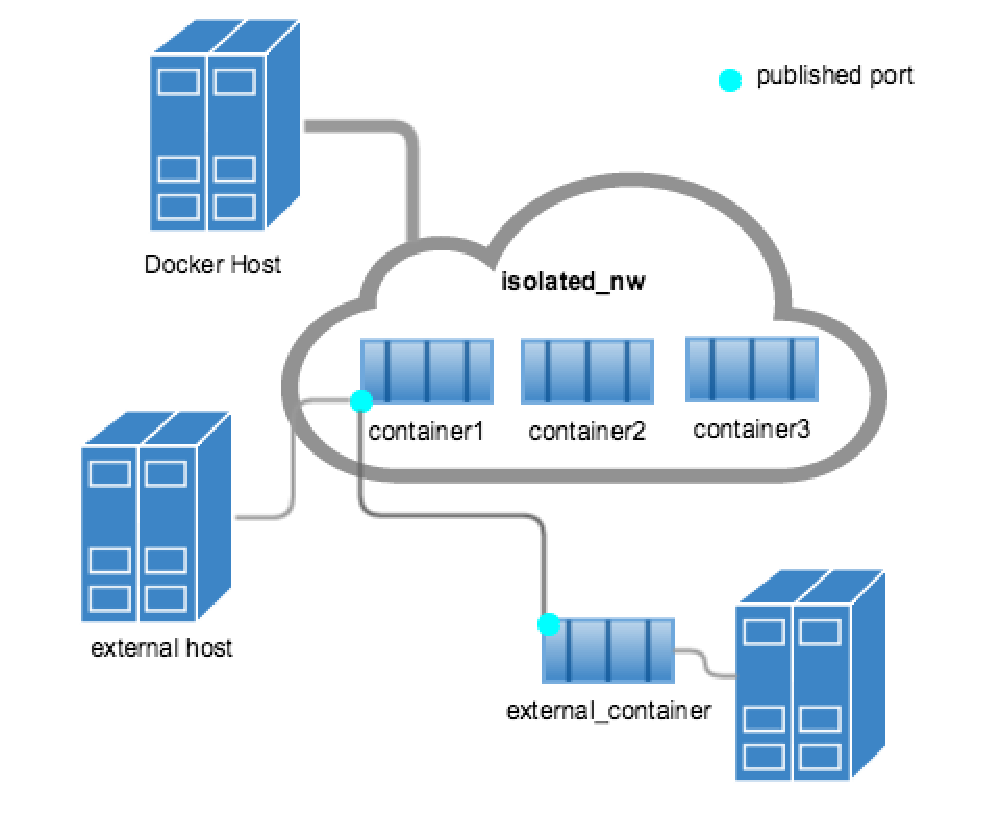
\includegraphics[width=0.7\linewidth]{figures/DockerPortPuEx}
	\caption[Docker Netzwerkzugriff]{Diagramm zur Darstellung des Docker Netzwerkzugriffs im User definierten Bridge-Netzwerk}
	\label{fig:dockerportpuex}
	\tiny{\quelle\url{https://docs.docker.com/engine/userguide/networking/}}
\end{figure}

Möchte man nun in einem Default oder User definierten Bridge-Netzwerk eines Host-Systems, wie in Abbildung \ref{fig:dockerportpuex} abgebildet, dass z. B. einzelne Container sich mit einem externem Host oder einem externen Container austauschen können, so ist ein \textit{Port exposing} und \textit{Publishing} notwendig.
Das \textit{Port exposing} erfolgt entweder durch Eintragung einer beliebigen Portnummer in Kombination mit dem Schlüsselwort \textbf{EXPOSE} im Dockerfile oder durch Ergänzung des \textit{docker run} Kommandos mit dem Flag \textit{{-}{-}expose}.

Für das \textit{Publishing} ist das Festlegen eines Ports im Dockerfile nicht möglich.
Stattdessen wird das \textit{docker run} Kommando durch das Flag \textit{{-}{-}publish} oder \textit{{-}{-}publish-all} ergänzt.
Dies teilt mit, welcher Port $>30000$ auf dem Host-System verfügbar ist.
Möchte man dennoch einen speziellen Port verwenden, so ist die Zuweisung des Ports erst zur Laufzeit möglich.

Aufgrund dessen, dass User definierte Bridge-Netzwerke vorrangig dafür verwendet werden kleinere Netzwerke auf einem Host zu erstellen, eignet sich diese Netzwerklösung nicht zur Umsetzung des Themas.
Dies liegt daran, dass Docker für diese Arbeit im Swarm Modus genutzt wird.
Hierbei handelt es sich um ein Cluster aus mehreren Docker-Engines.
Das Cluster besitzt mindestens einen Swarm-Manager.
Dieser nimmt Befehle für den Swarm entgegen und ermöglicht es, neue Swarm-Nodes, auch Swarm-Worker genannt, aber keine einzelnen Docker-Container zum Cluster hinzuzufügen.

Statt des User definierten Bridge-Netzwerks bietet Docker hierfür die Möglichkeit zur Erstellung eines Overlay-Netzwerks auf einem Swarm-Manager an.
Hierbei wird automatisch die Netzwerkbrücke \textit{docker\_gwbridge}, die zur Kommunikation zwischen den Swarm-Nodes verwendet wird, erstellt.
Diese Netzwerkbrücke wird zusätzlich immer dann angelegt, wenn ein gewöhnlicher Docker-Container keine Anbindung an ein externes Netz besitzt.
Der Swarm-Manager gewährt den einzelnen Swarm-Workern immer dann den Zugriff auf das Netzwerk, wenn die Swarm-Worker das Netzwerk zur Bewältigung ihrer Aufgaben benötigen. 

Bei der Erstellung des Overlay-Netzwerks ist zu beachten, dass die Docker-Engine im Swarm Modus arbeitet und der gewählte Swarm-Manager nicht an einen externen Key-Value-Store, wie z. B. ZooKeeper, angebunden ist.

Andernfalls spricht man von einem Overlay-Netzwerk ohne Swarm Modus.
Dieses wird in dieser Arbeit nicht weiter erläutert.
Einerseits, da es nicht erforderlich ist und andererseits, da Docker Inc. hierzu folgenden Satz in ihrem \glqq{}Docker container networking Guide\grqq{} verfasste:

\begin{quote}
	\textit{\glqq{}It may be deprecated in the future \cite{Docker:online3}.\grqq{}}
\end{quote}

\subsection{Volumes und shared Volumes}
\label{ss:sharedVolumes}
Wie bereits im Unterkapitel \ref{c:einführung} erwähnt, werden per default die Daten eines Containers in die writable Schicht des Docker-Containers geschrieben. 
Neben dem Nachteil, dass dieses Vorgehen die Container vergrößert, sind die darin abgelegten Daten lediglich zur Laufzeit des Containers verfügbar und werden nach der Ausführung gelöscht.

\begin{figure}
	\centering
	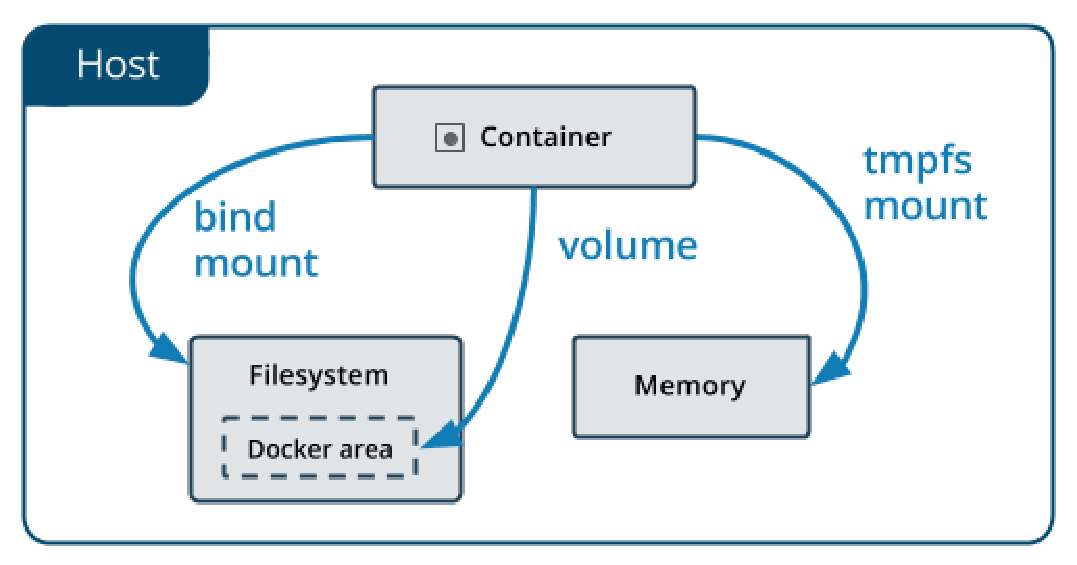
\includegraphics[width=0.7\linewidth]{figures/DockerMounts}
	\caption[Docker Mount Typen]{Übersicht der von Docker gebotenen Mount Typen}
	\label{fig:dockermounts}
	\tiny{\quelle\url{https://docs.docker.com/engine/admin/volumes/}}
\end{figure}

Aufgrund dessen bietet Docker zur dauerhaften Sicherung der Daten eines Containers, wie in Abbildung \ref{fig:dockermounts} gezeigt, die Verwendung von \textit{bind mounts}, \textit{tempfs mounts} und \textit{volumes} an.

Hierbei ist einerseits zu beachten, dass \textit{tempfs mount} vorrangig für Anwendungen mit hoher Performance oder sicherheitskritischen Daten genutzt wird und andererseits, dass Docker die Verwendung von \textit{bind mounts} in ihrer Dokumentation im Unterkapitel \glqq{}Use bind mounts\grqq{} für neu erstellte Anwendungen nicht empfiehlt. 
Somit wird lediglich die Datenspeicherung mit Hilfe von Volumes für die Anwendung verwendet und betrachtet.

Neben den Möglichkeiten zur Datensicherung geht aus Abbildung \ref{fig:dockermounts} hervor, dass das Volume in das Dateisystem eines Docker-Containers, im Swarm-Modus auch als Service bezeichnet, gemounted und der Inhalt auf dem Host-System (Windows oder Unix) gespeichert wird. 
Die Verwaltung des Volumes erfolgt entweder mittels des Docker \ac{CLI} oder der Docker API.

Aufgrund der Anforderung, dass die beiden erzeugten Volumes künftig von mehreren Services genutzt, beschrieben, gelesen und auf einem eigenen Host-System laufen sollten, konnten weder read-only noch lokale Volumes verwendet werden. 
Stattdessen wurden zwei shared Volumes durch Verwendung eines Volume Treibers realisiert.

Hierfür ist das Docker NFS, AWS EFS \& Samaba/CIFS Volume Plugin auf einem eigenen Host-System installiert worden.
Mit diesem wurde das Volume \textit{gatling-logs} erzeugt, das anschließend zu den Attack-Nodes und dem Reporter-Node der Anwendung gemountet wurde. 
Zusätzlich zum \textit{gatling-logs} ist das \textit{gatling-results} Volume erstellt worden. 
Dieses wurde im Reporter-Node und dem Report-Viewer Node des Swarms gemountet.

Somit verfügt der Reporter-Node über alle Daten des Angriffs und leitet diese per \textit{gatling-results} Volume an den Reporter-Viewer-Node, der für die Verwertung der Ergebnisse zuständig ist, weiter.

\chapter{Gatling - Test Framework}

In diesem Kapitel soll auf das Test Framework \textit{Gatling.io} eingegangen werden.
Im Besonderen wird analysiert, was Performance-Tests sind und welche Vorteile diese für den Entwickler bzw. die Softwarearchitektur mit sich bringen.

Nachdem mögliche Einsatzgebiete von Performance-Tests analysiert wurden, wird auf die \ac{DSL} von Gatling.io eingegangen.
Es werden hier die wichtigsten Befehle erläutert.

Gatling wurde am 20. Dezember 2011 erstmalig veröffentlicht und ist hauptsächlich in der Programmiersprache Scala implementiert. 
Laut der Plattform \textit{Open Hub}\footnote{{}Open Hub bietet eine detaillierte Übersicht über Open Source Projekte bzgl. der Aktivitäten, verwendeter Programmiersprachen usw. (vgl. \url{https://www.openhub.net})} hat Gatling über 50k Zeilen an Code bei mehr als 100 Contributors\footnote{{} Als Contributor ist ein Entwickler zu verstehen, der an dem Projekt selbstständig und freiwillig arbeitet.}.\cite{Gatli41:online} 
Das Tool wurde unter der Apache License 2.0 lizenziert.

\section{Performance-Tests}
\begin{figure}
	{\caption{Software Qualitätseigenschaften}
		\label{fig:ISO9126}}
	{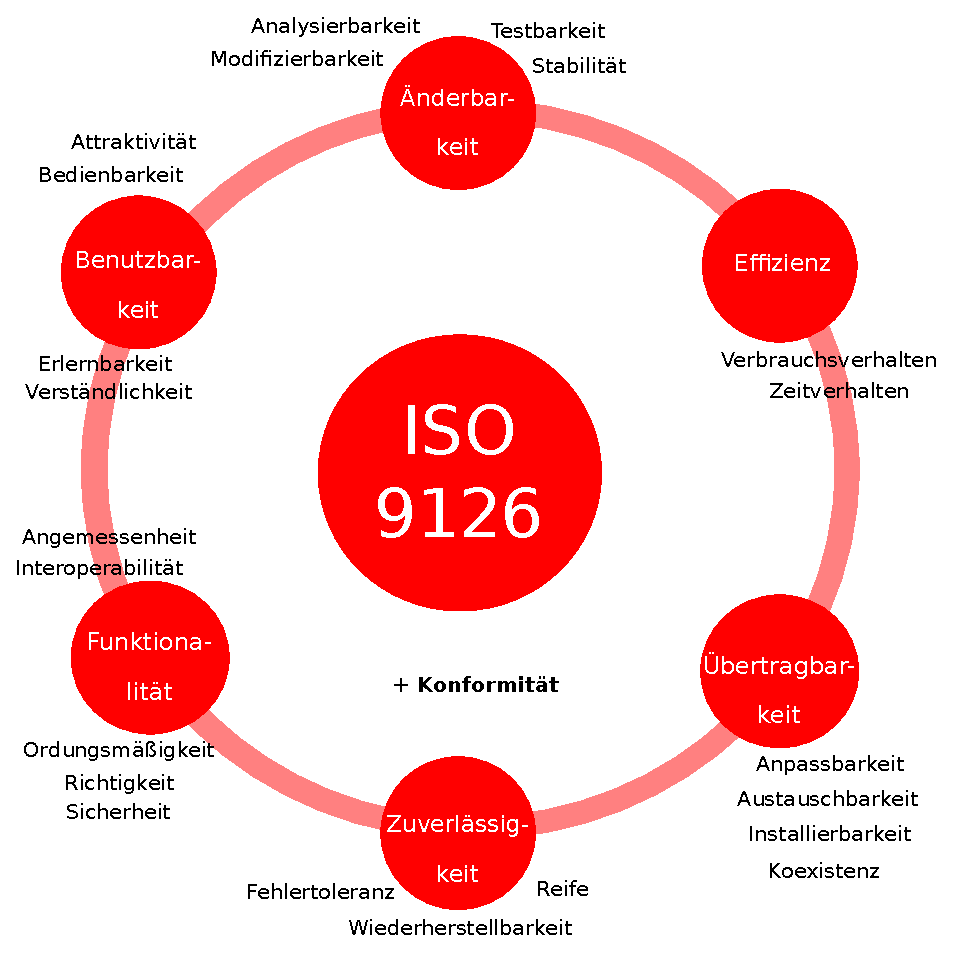
\includegraphics[scale=0.6]{\figdir/ISO9126}}\\
     \tiny{\quelle\url{https://commons.wikimedia.org/w/index.php?curid=52216179}\cite{ISO9126q74:online}}
\end{figure}
In der ISO 9126 wird geregelt wie die Softwarequalität einer Anwendung sichergestellt werden kann.\footnote{{} Die ISO 9126 wurde durch die ISO 25010 abgelöst - äquivalent dazu ist die DIN Norm 66272.}\cite{ISOIEC2533:online} 
Ein Punkt in der Norm ist \textit{Effizienz}, die in zwei Unterpunkte gegliedert ist:
\begin{itemize}
\item Zeitverhalten
\item und Ressourcenverbrauch.
\end{itemize}
Effizienz beschreibt das Verhältnis zwischen Leistungsniveau der Software und der verwendeten Betriebsmittel.
Das Zeitverhalten einer Anwendung beschreibt dabei die Antwort bzw. die Verarbeitungszeit oder auch den Durchsatz bei einer Funktionsausführung. 
Der Ressourcenverbrauch gibt den Status der verwendeten Betriebsmittel an, wie beispielsweise den verwendeten Speicher, die Netzwerklast bzw. Anzahl Festplattenzugriffe usw.

Mit Hilfe von Performance-Tests kann das erwartete Zeitverhalten einer Anwendung getestet werden. 
Durch diese Art der Tests können sogenannte \textit{Bottlenecks} der Anwendung ausfindig gemacht und beseitigt werden. 
Unter den \textit{Bottlenecks} versteht man einzelne Komponenten der programmierten Anwendung, die den gesamten Worfklow ausbremsen. 
Als Beispiel könnte folgende Situation dienen:
\begin{itemize}
    \item Eine aufwändigere Berechnung wurde in parallele Tasks ausgelagert
    \item Jeder der Tasks muss eine Datenbankabfrage durchführen, damit die aktuellsten Daten zur Verfügung stehen
    \item Durch diese langwierige Abfrage verzögert sich die gesamte Berechnung
\end{itemize}
Als Bottleneck ist hier die Abfrage zur Datenbank aufzuführen.
Diese sollte in einem vorgelagerten Prozess abgespalten werden. 
Auch wenn dieses konstruierte Beispiel sehr einfach und überzogen dargestellt ist, gibt es in echten Anwendungen auch Problembereiche, die vom Entwickler nicht als solche identifiziert werden konnten.
Beispielsweise könnte eine Abfrage an eine Schnittstelle unter normalen Bedingungen sofort erledigt sein, unter Last allerdings ändert sich deren Verhalten.
Ohne einen Test, der eine konstruierte Last bzw. Auslastung auf der Anwendung erzeugt, wird diese Art von Fehler nicht entdeckt.
Der Administrator kann so vorbeugend von Vornherein die Infrastruktur anpassen, bevor die Anwendung im produktiven Umfeld ist.
 
\subsection{Einsatzgebiete}

Als Einsatzgebiete sind zusammenfassend zu nennen:

\begin{itemize}
    \item Vorhersage von Engpässen (Bottlenecks) in Anwendungen:
   
    Durch einen Test, der eine simulierte Auslastung auf der Anwendung erzeugt, können einzelne Problembereiche der Anwendung aufgezeigt werden.
    
    \item Skalierung der Anwendung:

    Durch Performance-Tests kann eine beliebige Anzahl an Benutzern auf der Anwendung simuliert werden. Es könnte beispielsweise die Skalierung der Anwendung erprobt werden. Hier wird nicht nur die Softwarearchitektur des Programms getestet, sondern auch die IT-Infrastruktur. Durch die genannten Tests könnte beispielsweise aufkommen, dass ein Load-Balancer für eine erwartete Last von 1 Million Benutzern nicht ausreichend ist.
    
    \item Feedback für Benutzer verbessern:
    
    Der Benutzer der Anwendung bekommt ein besseres Produkt mit schnelleren Antwortzeiten, was insgesamt die Zufriedenheit beim Kunden/Benutzer verbessert.    
    
    \item Verbesserung/Optimierung der Software Architektur:
    
    Durch Erfahrungswerte aus vorhergehenden Tests kann langfristig die Softwarearchitektur angepasst bzw. verändert werden. Die Anwendung kann skalierbarer entworfen und geplant werden. Auch das Programmierverhalten der Entwickler wird dadurch positiv beeinflusst. Durch Erfahrungswerte können Fehler schon während der Entwicklungszeit aufgedeckt und verhindert werden. So werden Optimierungen während der Entwicklungsphase durchgeführt. 

\end{itemize}

\subsection{Herausforderungen bei Performance-Tests}

Wichtig bei Performance-Tests bzw. generell ist die genaue Definition eines zu erreichenden Ziels. 
Was genau soll als Ergebnis des Tests herausgefunden werden? Nur so kann die Testumgebung dementsprechend geplant und durchgeführt werden.\footnote{In der Praxis wird der Begriff \glqq Performance-Test\grqq{} äquivalent für Stress Tests bzw. Last Tests verwendet.\cite{Lasttest51:online}}

Performance-Tests sind abhängig von der zu erwarteten Leistung.
Sicherlich ist es nicht sinnvoll als \glqq kleines\grqq{} Startup mit einer Million von Requests zu rechnen.
Die Verhältnismäßigkeit von eingesetzter Architektur bzw. Betriebsmitteln zu der erwarteten Nutzungsintensität muss gegeben sein. 
Bei einem Performance-Test wird zwangsläufig irgendwann der Punkt kommen, an dem die Anwendung ein deutlich verlangsamtes Ansprechverhalten zeigt. 
Diesen Punkt muss jeder Software Ingenieur bzw. Manager individuell für das eigene Produkt passend wählen.

Es ist darauf zu achten, dass die Testbedingungen möglichst realistisch und ähnlich zu der Produktivumgebung zu wählen sind.
So muss beispielsweise beim Testen einer Anwendung auch berücksichtigt werden, dass es zu Verbindungsabbrüchen, unterschiedlichen Nutzungsarten, verschiedenen Clients und dergleichen kommen kann.
Um möglichst viele Szenarien testen zu können, muss im Vorfeld eine Analyse durchgeführt werden, wie die Anwendung hauptsächlich benutzt werden wird.
So können Parameter wie die erwartete Benutzerzahl, verwendete Client Konfigurationen usw. herausgefunden und getestet werden.

\section{Gatling - Features}

%https://gatling.io/docs/current/cheat-sheet/

\subsection{Gatling DSL}

Unter einer \acf{DSL} versteht man eine Beschreibungssprache für ein definiertes Problemfeld. 
Sie erleichtert die Interaktion mit einem komplexen System ohne die genauen Hintergründe zu kennen.
Die Lesbarkeit bzw. das Bedienverhalten kann so deutlich verbessert werden. 
Für Gatling wurde eine eigene \ac{DSL} entworfen, um die Test Szenarios so lesbar wie möglich zu gestalten. 
In Tabelle \ref{table_cheatSheetDSL} sind die wichtigsten Befehle mit deren Bedeutungen aufgelistet.\footnote{{} Für eine vollständige Auflistung der Befehle: vgl. \url{https://gatling.io/docs/current/cheat-sheet/} (Stand der Abfrage: 18.12.2017)} 
Ein Code Beispiel für die Verwendung dieser Schlüsselwörter wird in Kapitel \ref{sec:testWithGatlingExample} in Beispiel \ref{testCodingSample} gegeben. 

\begin{table}[]
\centering
\caption{Cheat-Sheet DSL Gatling.io}
\label{table_cheatSheetDSL}
\begin{adjustbox}{max width=\textwidth}
\begin{tabular}{|c|c|}
\hline
\rowcolor[HTML]{FFCB2F} 
\textbf{Befehl} & \textbf{Verwendung} \\ \hline
scenario &  definiert ein neues zu testendes Szenario\\ \hline
repeat & gibt die Anzahl an, wie oft ein Test ausgeführt werden soll \\ \hline
exec \& get & es wird die genaue \ac{URI} angegeben, die getestet wird  \\ \hline
setUp - Methode & definiert die Testumgebung \\ \hline
inject - Methode & gibt an wie viele Benutzer auf der Anwendung simuliert werden sollen\footnote{{} Hier können verschiedene Parameter mitgegeben werden, wie beispielsweise 100 Benutzer auf einmal oder ein stetiger Anstieg der Benutzer zu einem konfigurierten Maximalwert.}  \\ \hline
Feeder Definition & gibt verschiedene Modi für den Import in das Test Szenario ein \\ \hline
HTTP Action & definiert die Parameter, die für einen erfolgreichen Request gesetzt werden müssen \\ \hline
HTTP Checks & checkt den Rückgabewert des HTTP Requests  \\ \hline
Assertions &  die erwarteten Ergebnisse werden mit den tatsächlichen abgeglichen\footnote{{} Auch hier können verschiedene Einstellungen wie Scopes, Bedingungen usw. getätigt werden. } \\ \hline


\end{tabular}
\end{adjustbox}
\end{table}

\subsection{Metriken}

Gatling.io sammelt nach erfolgreichem Testen einer Anwendung die gemessenen Metriken in einem Bericht und stellt diese dem Benutzer zur Verfügung. 
In Abbildung \ref{fig:gatlingMetriken} ist exemplarisch ein Bericht aufgezeigt. 
In der Übersicht ist in einem Säulendiagramm das Antwortverhalten gegliedert, bspw. grüner Balken hat eine Antwortzeit von unter 800 ms. 
Außerdem lässt sich erkennen wie viele Requests insgesamt durchgeführt wurden, wie viele fehlgeschlagen sind sowie die erfolgreich beantworteten Requests.
\begin{figure}
	{\caption{Gatling Metriken}
		\label{fig:gatlingMetriken}}
	{\includegraphics[scale=0.3]{\figdir/gatlingMetriken}}\\
	\tiny{\quelle\url{https://gatling.io/wp-content/uploads/2016/12/rapport.png}}
\end{figure}



\section{Continous Integration}

\begin{figure}
	{\caption{Continous Integration Prozess}
		\label{fig:continousIntegration}}
	{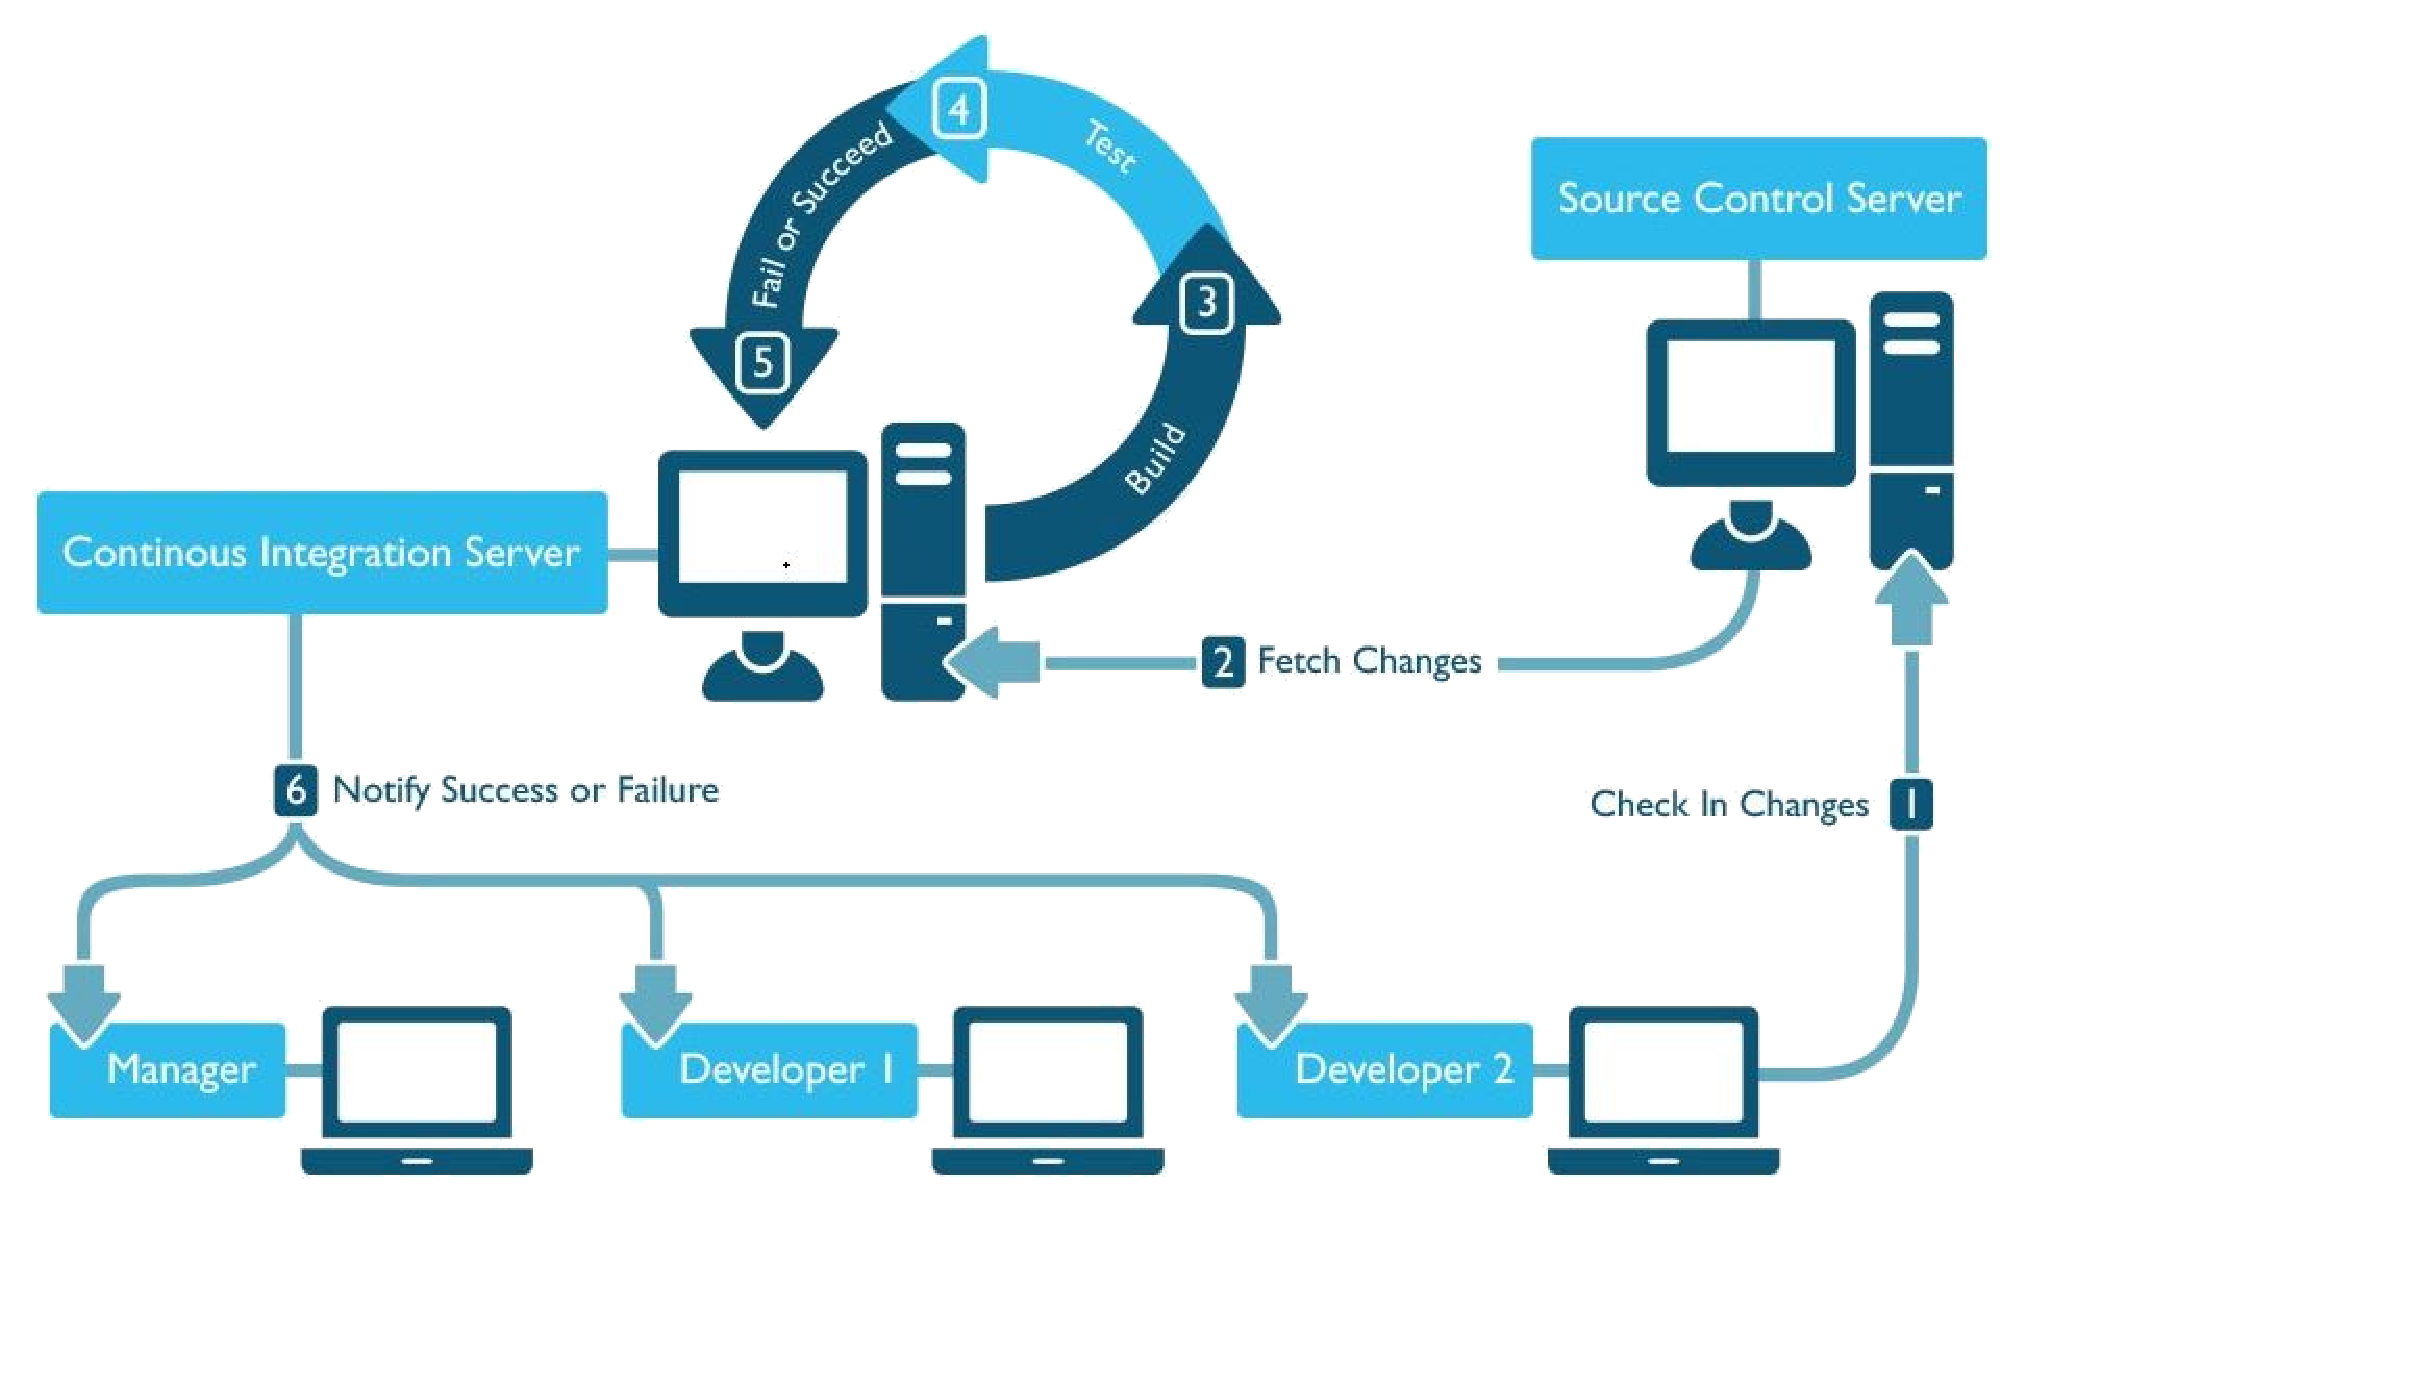
\includegraphics[scale=0.5]{\figdir/CI}}
	\tiny{\quelle\url{http://www.anarsolutions.com/making-ci-effective-size-organization/}}
\end{figure}

Der Einsatz von Buildservern in einer Continous Integration Umgebung gehört mittlerweile zu den Standard Werkzeugen eines Entwicklerteams. 
Aber was ist Continous Integration und wie können Lasttests in diesen Prozess eingebunden werden?

In Abbildung \ref{fig:continousIntegration} ist ein typischer Continous Integration Prozess dargestellt. 
Die Entwickler pushen ihren modifizierten Sourcecode in den Source Control Server.
Dieser kann ein GIT Repository oder ein ähnliches Tool wie \ac{TFS} der Firma Microsoft sein.
Dann kommt der eigentliche Buildserver ins Spiel.
Dieser holt die vorgenommen Änderungen vom Source Control Server und versucht das Projekt zu kompilieren.
Anschließend werden die definierten Tests ausgeführt und sowohl im Erfolgs- als auch im Fehlerfall die Entwickler bzw. Teamleiter informiert.
Die Meldung, dass der Vorgang erfolgreich durchgeführt wurde, wird langfristig wahrscheinlich überflüssig.
Als Mittelweg wäre empfehlenswert, dass nach einem fehlgeschlagenen Versuch der erstmalige erfolgreiche Vorgang als Erfolgsmeldung übermittelt wird.
Durch diesen Prozess bekommen die Entwickler schnelles Feedback in Fehlerfällen und können diese beheben.

Abbildung \ref{fig:jenkinsBuildResult} zeigt einen Graphen, der auf dem Buildserver \glqq Jenkins\grqq{} während eines Buildvorgangs generiert wurde.
Die Grafik zeigt den \glqq Performance Trend\grqq{} einer Anwendung über mehrere Analysen hinweg.
Wie aus dem Graph entnommen werden kann, gab es zwischen dem achten und zehnten Buildvorgang stetige Performance Probleme, die aber dann im elften Buildvorgang gelöst werden konnten.
So wurden potentielle Bottlenecks, die unabsichtlich durch den Entwickler eingebaut wurden, entdeckt und konnten nach dem Buildvorgang behoben werden.
Die Anwendung war nicht im Produktivbetrieb, als diese Fehler entdeckt und behoben wurden.
Diese Tatsache zeigt den klaren Vorteil von Performance-Tests in einem Continous Integration Prozess auf, da die Fehler automatisch noch vor dem Release der Software entdeckt und behoben werden können.
\begin{figure}
	{\caption{Ergebnis der Analyse am Jenkins Buildserver}
		\label{fig:jenkinsBuildResult}}
	{\includegraphics[scale=0.3]{\figdir/jenkinsResult}}\\~\\
				\tiny{\quelle\url{https://gatling.io/wp-content/uploads/2016/12/jenkins2.png}}
\end{figure}


\section{Anwendungsfall - Performance-Test mit Gatling}
\label{sec:testWithGatlingExample}
In diesem Unterkapitel soll auf den grundsätzlichen Aufbau eines Gatling Tests eingangen werden.

Gatling Tests sind in der Programmiersprache Scala\footnote{{} Scala ist eine Java-ähnliche Sprache, die auf der \ac{JVM} läuft.} implementiert.
Im Code-Beispiel \ref{testCodingSample} ist beispielhaft ein solcher Test dargestellt.
Dieser soll die Schnittstelle für das zufällige Abholen eines Witzes auf Last testen.
Die grundsätzliche Funktionsweise der Schnittstelle wird an dieser Stelle vorausgesetzt.
Dies muss im Vornherein durch Unit - bzw. Integrationstests sichergestellt werden.
Für das Testen der Auslastung müssen allerdings einige Details über die Schnittstelle bekannt sein.
So muss u.a. der Server mit zugehörigem Port sowie der genaue Aufbau der Schnittstelle für den Entwickler einsehbar sein.
Dieser Aspekt wird an dieser Stelle erwähnt, da es in größeren Unternehmen durchaus sein könnte, dass unabhängige Teams die gleiche Anwendung testen müssen.
In diesem Fall hätte der Entwickler des Performance-Tests nur die Black-Box-Sicht auf die bereits programmierte Anwendung.
Das Code Beispiel \ref{testCodingSample} soll nun im Detail erläutert werden.

Zuerst werden die notwendigen Bibliotheken über \glqq Import-Befehle\grqq{} geladen.
Die Klasse \glqq RandomJokeSimulation\grqq{} erbt von der definierten Klasse \glqq Simulation\grqq{}.\footnote{{} Jeder Gatling.io Test muss von der Simulation Klasse erben.}
Anschließend wird die Verbindung konfiguriert sowie der notwendige Test-Request zusammengebaut.
In diesem Beispiel läuft die Anwendung im internen Netz an der Adresse \glqq http://192.168.111.20\grqq{} auf Port 58080.
Damit der Request vom Server akzeptiert wird, werden die notwendigen Header gesetzt.

Anschließend wird die zu testende Logik, in Gatling.io \glqq Scenario\grqq{} genannt, implementiert.
Das Scenario bekommt einen Namen zugewiesen und die Aufforderung, wie oft dieses ausgeführt werden soll.
Zudem wird der genaue Pfad der Schnittstelle definiert und die \ac{HTTP} Methode, die auf die \ac{REST} Schnittstelle ausgeführt werden soll, ausgewählt.

Der Lasttest soll möglichst unter den Bedingungen durchgeführt werden, die auch im produktiven System aktiv sind.
So ist es unrealistisch anzunehmen dass 1000 Benutzer exakt zeitgleich die Abfrage auf die Schnittstelle absetzen.
Es ist vielmehr anzunehmen, dass die Benutzeranzahl mit zunehmender Laufzeit des Programms ansteigen wird.
Genau diese Funktionalität bietet Gatling.io an.
Zur Testlaufzeit können kontinuierlich, dies ist konfigurierbar, neue Benutzer erstellt werden, die auch Abfragen auf die Schnittstelle absetzen.
So kann ein realistischer Use-Case getestet werden.

\begin{minipage}{\linewidth}
\begin{lstlisting}[frame=single,caption=Testabfrage auf Schnittstelle in Gatling, label=testCodingSample, language=Scala]
import io.gatling.core.Predef._
import io.gatling.http.Predef._
import scala.concurrent.duration._

class RandomJokeSimulation extends Simulation {
    val httpConf = http
        .baseURL("http://192.168.111.20:58080")
        .acceptHeader("application/json")
        .acceptEncodingHeader("gzip, deflate")
        .userAgentHeader("Mozilla/5.0 (Windows NT 5.1; rv:31.0) Gecko/20100101 Firefox/31.0")

    val scn = scenario("RandomJokeSimulation").repeat(100) {
        exec(http("getRandomJoke")
        .get("/api/v1/joke/random"))
    }    

    setUp(
        scn.inject(atOnceUsers(100))
    ).protocols(httpConf)
}
\end{lstlisting}
\end{minipage}
Als Alternative zu Gatling.io ist \textit{Apache JMeter} zu nennen.\footnote{{} vgl. \url{https://jmeter.apache.org/}}
JMeter wurde im Jahr 1998 erstmalig veröffentlicht und wurde hauptsächlich in Java implementiert.\footnote{{} Der direkte Vergleich von JMeter zu Gatling ist hier aufgezeigt.\cite{JMetervs63:online}}

\section{Zwischenfazit Lasttests}

Performance- oder Lasttests sind notwendig um eine stabile Anwendung bzw. API zu entwickeln.
Langfristig wird sich die Architektur bzw. der Programmierprozess verbessern, wenn die Ergebnisse der Tests analysiert, ausgewertet und auch für zukünftige Entwicklungen berücksichtigt werden.
Durch die Integration in eine Continuous Integration Umgebung wird ein schnelles Feedback der Tests an die Entwickler garantiert und diese können noch während der Entwicklungsphase aufkommende negative Trends bzgl. der Antwortzeiten oder der Performance der Anwendung analysieren und beheben.
So wird garantiert, dass eine umfangreich getestete Software keine bösen Überraschungen bei aufkommender Last zeigt.
Mit Gatling wird ein umfangreiches Performance-Test Tool angeboten, das sowohl eine gute Integration in einen Buildserver, wie beispielsweise Jenkins bietet, als auch mit einer \ac{GUI} einfach Operationen durchführen lässt.



\chapter{Kubernetes}

\section{Einführung}

\section{Architektur}

\section{Skalierung}

\section{Persistenz}

\section{Service Discovery und Load Balancing}

\section{Batch Exectution}
\chapter{Jericho}

Jericho ist der Arbeitstitel des Proof-of-Concept Gatling Lasttests mit Hilfe von Docker Containern durchzuführen.
Wie in Kapitel \ref{c:docker} beschrieben eignen sich Docker Container sehr gut dafür Software zu paketieren, da ein Container einerseits alle notwendigen Abhängigkeiten mitbringen und andererseits nach Verwendung auf einen definierten Startzustand zurückgesetzt werden kann.

Weitere Vorteile von Containern im Kontext von Lasttests sind die bereits erwähnte horizontale Skalierbarkeit und das Ressourcenmanagement.
Ersteres ermöglicht es einerseits höhere Lasten zu erzeugen aber auch andererseits die dynamische Skalierung der Anwendung um Testen zu können, wie stark man die Anwendung skalieren muss um die erwartete Last verarbeiten zu können.
Zweiteres kann nützlich sein, wenn man bspw. ermitteln will wie viel Leistung ein Container oder eine \ac{VM} benötigt, wenn die erwartete Last in etwa bekannt ist.
Dies unterstützt die Entwickler bei der Kostenkalkulation im Rahmen von Cloud-Hosting (AWS, Azure, etc.)

\section{Architektur}

Das Projekt Jericho besteht aus den drei folgenden Container-Typen:

\begin{itemize}
	\item Attack-Container
	\item Repoter-Container
	\item Report-Viewer-Container
\end{itemize}

Wobei nur die \textit{Attack-Container} skaliert werden müssen.
Von den beiden anderen Typen sollte jeweils immer nur eine Instanz gestartet werden.

\subsection{Attack-Container}

Das \textit{Attack}-Container-Image basiert auf dem offiziellen Java-Image \textit{openjdk:8-jdk-alpine}.
Zusätzlich wird in dem Container Gatling installiert und ein kleines Bash-Skript ergänzt, welches beim Container-Start ausgeführt wird.

Das Skript \textit{attacks.sh} beinhaltet im Wesentlichen vier Schritte:

\begin{enumerate}
	\item Soweit vorhanden l\"oschen von Ergebnissen vorheriger Testl\"aufe aus dem Shared Volume \textit{gatling-logs} (vgl. Abschnitt \ref{ss:sharedVolumes}).
	\item Starten von Gatling mit einigen \ac{CLI}-Switches um zu gew\"ahrleisten, dass keine User-Interkation notwendig ist wenn ein Testlauf gestartet wird.
	\item Verschieben der aktuellen Test-Ergebnisse in das Shared Volume \textit{gatling-logs}. Die Log-Datei wird dabei umbenannt um Dateinamenkonflikte mehrerer Attack-Container zu vermeiden.
	\item Blockieren des Containers durch einen ewigen \glqq{}sleep\grqq{} um zu vermeiden, dass der Container von einem Clustermanagementsystem neu gestartet wird, sobald er sich beendet.
\end{enumerate}

Der Container ist dabei so entworfen, dass auszuf\"uhrende Simulationen im Default-Verzeichnis \textit{/opt/gatling/user-files/simulations/} abgelegt werden \textbf{m\"ussen}.
Es gilt au\ss{}erdem zu beachten, dass niemals mehr als eine Simulation (vgl. Abschnitt \ref{sec:testWithGatlingExample}) in dem Verzeichnis abgelegt werden darf, da Gatling ansonsten in einen interaktiven Modus wechselt um zu erfragen welche Simulation ausgef\"uhrt werden soll.

\subsection{Reporter-Container}

Auch das \textit{Reporter}-Container-Image basiert auf dem offiziellen Java-Image \textit{openjdk:8-jdk-alpine}, enth\"alt eine Gatling-Installation und ein spezielles Start-Skript.
Im Gegensatz zum Attack-Container, der je nach Bedarf mehrmals gestartet werden kann, sollte vom Reporter-Container nur eine Instanz gestartet werden.
Der Reporter-Container \"ubernimmt die Aufgabe alle Ergebnisse der Attack-Container zu analysieren und in einen HTML-Report zu aggregieren.
Zu diesem Zweck \"uberwacht er den Inhalt des Shared Volume \textit{gatling-logs} und im Fall einer \"Anderung wird der HTML-Report neu erzeugt.
Um \"Anderungen zuverl\"a\ss{}ig erkennen zu k\"onnen wird im Abstand von 10s der gesamte Inhalt des Shared Volume mit Hilfe des Linux-CMDlets \textit{tar} in einen Dateistream geschrieben, von welchem dann ein MD5-Hash\footnote{nat\"urlich k\"onnte man auch andere Hashing-Verfahren nutzen aber MD5 bietet in diesem Fall eine ausreichende Kollisionssicherheit im Verh\"altnis zur ben\"otigten Leistung.} erzeugt wird.
\"Andert sich der Hashwert, wird der HTML-Report neu erzeugt.

Der HTML-Report wird im Shared Volume \textit{gatling-results} abgelegt, damit der Report-Viewer-Container diesen ausliefern kann.

\subsection{Report-Viewer-Container}

Der letzte Container-Typ ist optional und wurde auch nicht f\"ur das Projekt speziell modifiziert.
Der Report-Viewer-Container ist ein Container vom Image \textit{nginx:1.13-alpine} und lediglich der Auslieferung des HTML-Reports.
Alternativ h\"atte man auch in den \textit{Reporter}-Container einen Web-Server integrieren oder die Ergebnisse auf einen externen Persistenz-Layer (vgl. Abschnitt \ref{ss:sharedVolumes}) \"ubertragen k\"onnen.

\section{Deployment}

W\"ahrend der Projektphase wurde der \glqq{}Jericho-Stack\grqq{} auf die folgenden zwei Arten benutzt:

\begin{itemize}
	\item Lokal mit Hilfe von Docker-Compose (vgl. Abschnitt \ref{ss:dockerCompose}).
	\item In einem Docker Swarm basiertem Cluster.
\end{itemize}

Die ben\"otigten Konfigurationsdateien f\"ur Docker-Compose und Docker Swarm sind sich sehr \"ahnlich, weshalb die Wahl von Docker Swarm als Clustermanagementsystem f\"ur die Testumgebung nahe lag.
Die zwei gravierensten Unterschiede zwischen einem Docker-Compose und einem Docker Swarm basierten Deployment sind die Persistenz der Container und die Bereitstellung der Simulationen.
Da die Problematik der Persistenz bereits in Kapitel~\ref{c:docker} behandelt wurde, wird in diesem Abschnitt darauf verzichtet.

Die Bereitstellung der Simulationen kann bei einem lokalen Deployment mit Docker-Compose verh\"altnism\"a\ss{}ig einfach durch einen Volume-Mount der Datei in das Zielverzeichnis gel\"ost werden.
Bei einem Deployment in einem Docker Swarm Cluster ist dies nur unter bestimmten Bedingungen m\"oglich.
Unter anderem sind folgende Varianten zur Umsetzung denkbar:

\begin{itemize}
	\item Die Simulationsdatei wird auf allen Cluster-Mitgliedern im selben Pfad abgelegt, so dass sie unabh\"angig davon auf welchem Host ein Attack-Container gestartet wird verf\"ugbar ist.
	\item Durch ein sogenanntes \textit{Placement Constraint} werden alle Attack-Container auf einer Cluster-Node, auf der auch die Simulationsdatei vorhanden ist erzeugt. Dies kann zu Performance-Problemen f\"uhren und sollte daher vermieden werden.
	\item Die Simulationsdatei wird durch ein read-only Shared Volume allen Attack-Nodes bereitgestellt. Dieses Shared Volume sollte z.B. mit dem bereits erw\"ahnten \textit{Docker NFS, AWS EFS \& Samaba/CIFS Volume Plugin} erzeugt werden, damit es unabh\"angig vom aktuellen Host verf\"ugbar ist.
	\item Docker Swarm bietet einen speziellen Mechanismus zur Bereitstellung von Konfigurationsdateien, der durch das CMDlet \textit{docker config} kontrolliert wird. Mit diesem k\"onnen entweder einzelne Values oder auch ganz Dateien in einem Docker Swarm internen Key-Value-Store abgelegt und beim Deployment mit Hilfe eines Mount-Point den Containern zur Verf\"ugung gestellt werden. Diese Variante wurde w\"ahrend des Projekts benutzt, da sie auch bequem remote benutzt werden kann ohne z.B. mit NFS oder SCP Dateien auf einen Server \"ubertragen zu m\"ussen.
\end{itemize}

Die zum Einsatz gekommenen Konfigurationsdateien sowohl f\"ur das lokale als auch das Cluster basierte Deployment sind im Anhang zu finden.
W\"ahrend die Docker-Compose Konfigurationen kaum einer Anpassung bed\"urfen (abgesehen von dem Mount-Point f\"ur die Simulationsdatei) m\"ussen f\"ur das Deployment auf einen Docker Swarm einige Vorbereitungen getroffen werden.
Eine genaue Beschreibung w\"urde allerdings den Rahmen dieser Arbeit sprengen.
Bei Interesse gibt das Projektteam gerne Auskunft dar\"uber welche Schritte im Detail durchgef\"uhrt werden m\"ussen.

\section{Demo-Anwendung}

Um die beschriebene Zusammenstellung von Containern testen zu k\"onnen bedurfte es einer Testanwendung, die unkompliziert bereitgestellt werden kann, \"uber eine REST-API verf\"ugt und bestenfalls sogar skaliert werden kann.
Auf eine REST-API h\"atte ggf. auch verzichtet werden k\"onnen allerdings ist es deutlich einfacher eine REST-API zu testen als eine vollst\"andige Web-Applikation, da bei ersterer nur primitive JSON-Objekte empfangen und versendet werden m\"ussen statt Form-POSTs und umst\"andliche Query-Strings zu generieren, parsen und verarbeiten zu m\"ussen.

Um volle Flexibilit\"at genie\ss{}en und auf eventuelle zus\"atzliche Anforderungen reagieren zu k\"onnen wurde eine Demo-Anwendung mit Hilfe des Frameworks Vert.x~\cite{Vertx:online} implementiert.
Die Anwendung und ihre API ist der ICNDB~\cite{ICNDB:online} nachempfunden und benutzt als Persistence Layer eine PostgreSQL Datenbank.

Das Deployment der Demo-Anwendung wurde auch mit Docker realisiert wodurch es allen Projekt-Teilnehmern erm\"oglicht wurde die Anwendung ohne ein aufwendigeres Setup benutzen zu k\"onnen.

\chapter{Tests und Bewertung}

Nach Fertigstellung des Proof-of-Concepts wurde eine Reihe von Tests mit unterschiedlichen Konfigurationen durchgef\"uhrt um die Auswirkungen verschiedener Parameter auf die Ergebnisse des Lasttests der Demo-Anwendung beobachten zu k\"onnen.
Bei der Testreihe wurden folgende Parameter variiert:

\begin{itemize}
	\item Anzahl der Attack-Container (1-6 Instanzen)
	\item Anzahl der Demo-App-Container(1 oder 3 Instanzen)
	\item Anzahl der parallelen User (300, 600 oder 1000)
	\item Anzahl der Requests, die jeder User ausf\"uhrt (300, 500 oder 800)
\end{itemize}

\section{Interpretation der Testergebnisse}
\label{s:valuationInterpretation}

Tabelle \ref{tbl:testResults} zeigt die aggregierten Ergebnisse der Testreihe.
F\"ur die folgenden Beobachtung wird die erste Testreihe, bei der nur 1 Demo-App Container vorhanden war zun\"achst au\ss{}en vor gelassen.

Das Zeitverhalten in Abh\"angigkeit zur Anzahl der parallelen User und der Anzahl der Attack Container ist mehr oder weniger wie erwartet.
So verdoppelt sich das 99\% Quantil und die durchschnittliche Antwortzeit in etwa, bei der Steigerung der User von 300 auf 1000 bei 1 Attack Container.
Nahezu direkt proportional ist das Verh\"altnis wenn man die Steigerung der Anzahl von Usern bei jeweils 6 Containern betrachtet.

Interessanter ist wie sich der Durchsatz der Anwendung ver\"andert.
Egal ob nun bei 600 oder 1000 parallele User oder ob diese jeweils 500 oder 800 Requests ausf\"uhren, die durchschnittliche Anzahl von Requests die pro Sekunde verarbeitet werden verh\"alt sich indirekt proportional zur Anzahl der Attack-Container.

Die erste Testreihe bei der nur ein Demo-App Container verf\"ugbar war widerspricht diesen Beobachtungen interessanterweise.
So ist es bei dieser Testreihe schwierig eine Tendenz des Durchsatzes festzustellen.
Das Zeitverhalten bleibt aber auch bei dieser Testreihe mehr oder minder im Erwartungsrahmen.
So verh\"alt sich sowohl das 99\% Quantil als auch die durchschnittliche Antwortzeit proportional zur Anzahl der Attack Container.
M\"ogliche Ursachen f\"ur die Unsch\"arfen bei den Testwerten und allgemeine Probleme werden im Abschnitt~\ref{s:valuationProblems} diskutiert.

Leider enth\"alt der von Gatling erzeugte HTML-Report nicht die Gesamtzeit, die eine Simulation in Anspruch genommen hat.
Daher l\"asst sich die These der Gruppe, dass die Anzahl der Requests, die jeder User w\"ahrend einer Simulation ausf\"uhrt, sich nur auf die Dauer der Simulation nicht aber auf Durchsatz oder Zeitverhalten auswirkt nur anhand der Log-Dateien zweifelsfrei nachweisen.
Da diese aber sehr umfangreich sind (mehr als 2GB f\"ur die in Tabelle~\ref{tbl:testResults} gezeigte Testreihe) wird im Weiteren darauf verzichtet.

\section{Probleme der Auswertung}
\label{s:valuationProblems}

W\"ahrend der Durchf\"uhrung der Testreihe zeigte sich wiederholt das Verhalten, dass bei $n$ gestarteten Container $n-1$ Container verh\"altnism\"a\ss{}ig schnell gestartet wurden, der n-te Container aber unverh\"altnism\"a\ss{}ig lang ben\"otigte um vom Cluster bereitgestellt zu werden.
Das Test-Cluster bestand aus 3 Nodes, die alle gleichm\"a\ss{}ig belastet werden sollten.
Es wurde keine gesonderte Konfiguration vorgenommen um das Platzierungsverhalten der Container irgendwie zu beeinflussen.
Da alle ben\"otigten Container Images bereits vor der Testreihe auf allen Hosts verf\"ugbar waren scheidet auch die Begr\"undung aus, dass einer der Hosts das Image noch herunterladen musste.
Auch ein Neustart aller Hosts, das entfernen aller Images und einige andere Versuche \"anderten nichts an diesem Verhalten.

Leider k\"onnte dieses Verhalten allerdings einige Kennzahlen durchaus beeintr\"achtigen.
Speziell unter der Pr\"amisse, dass bei weniger Requests pro User die Simulation sehr schnell abgeschlossen ist, k\"onnte es zu F\"allen kommen, dass gar nicht alle Container echt parallel die Demo-Applikation unter Last setzen.
Dies betrifft im Besonderen die erste Testreihe, bei der nur jeweils 300 Requests pro User ausgef\"uhrt wurden.
Auch deshalb wurde diese Testreihe im Abschnitt~\ref{s:valuationInterpretation} gesondert behandelt.

\afterpage{%
	\clearpage
	\thispagestyle{empty}
	\begin{landscape}
		\begin{table}[]
		\centering
		\caption{Test-Ergebnisse von Jericho}
		\label{tbl:testResults}
		\begin{tabular}{|l|l|l|l|l|l|l|l|}
		\hline
Demo-App  Container & Attack Container & Parallele User & Requests/User & Requests gesamt & Mean Requests/s & 99\% Quantil & Mean \\ \hline
1                   & 1                & 300            & 300           & 90.000          & 6.923           & 106          & 39   \\ \hline
1                   & 2                & 300            & 300           & 180.000         & 7.200           & 130          & 62   \\ \hline
1                   & 3                & 300            & 300           & 270.000         & 5.510           & 143          & 65   \\ \hline
1                   & 4                & 300            & 300           & 360.000         & 7.500           & 172          & 74   \\ \hline
1                   & 5                & 300            & 300           & 450.000         & 7.627           & 294          & 78   \\ \hline
1                   & 6                & 300            & 300           & 540.000         & 7.200           & 302          & 183  \\ \hline
3                   & 6                & 300            & 300           & 540.000         & 6.067           & 429          & 251  \\ \hline
3                   & 1                & 600            & 500           & 300.000         & 8.823           & 177          & 62   \\ \hline
3                   & 2                & 600            & 500           & 600.000         & 7.142           & 184          & 160  \\ \hline
3                   & 3                & 600            & 500           & 900.000         & 7.627           & 303          & 183  \\ \hline
3                   & 4                & 600            & 500           & 1.200.000       & 6.382           & 469          & 305  \\ \hline
3                   & 5                & 600            & 500           & 1.500.000       & 7.317           & 528          & 338  \\ \hline
3                   & 6                & 600            & 500           & 1.800.000       & 6.451           & 743          & 489  \\ \hline
3                   & 1                & 1.000          & 800           & 800.000         & 9.411           & 206          & 102  \\ \hline
3                   & 2                & 1.000          & 800           & 1.600.000       & 7.373           & 353          & 255  \\ \hline
3                   & 3                & 1.000          & 800           & 2.400.000       & 7.843           & 466          & 344  \\ \hline
3                   & 4                & 1.000          & 800           & 3.200.000       & 7.002           & 733          & 523  \\ \hline
3                   & 5                & 1.000          & 800           & 4.000.000       & 7.299           & 900          & 655  \\ \hline
3                   & 6                & 1.000          & 800           & 4.800.000       & 6.916           & 1.113        & 836  \\ \hline
		\end{tabular}
		\end{table}
	\end{landscape}
\clearpage
}

\chapter{Fazit}



\appendix
\chapter*{Abkürzungen}
\begin{acronym}
\acro{Demo}{Demo Abkürzung}



\end{acronym}
\chapter{Anhang}
%Do not display source code chapters in toc
\addtocontents{toc}{\protect\setcounter{tocdepth}{0}}


\addtocontents{toc}{\protect\setcounter{tocdepth}{2}}

\chapter{Verzeichnisse}
\listoffigures
\cleardoublepage
\lstlistoflistings
\cleardoublepage
\listoftables
\cleardoublepage



\bibliographystyle{natger}
\bibliography{thesis}

\footnotesize


\end{document}
